\documentclass{llncs}
\pagestyle{plain} % turn on page numbers in llncs

\usepackage{isabelle,isabellesym}
\usepackage{latexsym}
\usepackage{amssymb}

% this should be the last package used
\usepackage{pdfsetup}

\newtheorem{thm}{Theorem}

% no right margin in quote:
\renewenvironment{quote}
{\list{}{}%
\item\relax}
{\endlist}

\newcommand{\noquotes}[1]{{\renewcommand{\isachardoublequote}{}\renewcommand{\isachardoublequoteopen}{}\renewcommand{\isachardoublequoteclose}{}#1}}

\isabellestyle{it}

\renewcommand{\isacharunderscore}{\_}
\renewcommand{\isacharunderscorekeyword}{\_}
\renewcommand{\isadigit}[1]{{\rm #1}}

% for uniform font size
\renewcommand{\isastyle}{\isastyleminor}

\newcommand{\eqnum}{\refstepcounter{equation}\hfill(\theequation)}

\hyphenation{Isa-belle}


\begin{document}

\title{Title}
\author{Author}
\institute{Technische Universit\"at M\"unchen}
\date{}
\maketitle

\begin{abstract}
Abstract
\end{abstract}


\section{Introduction}

All proofs have been formalized in the theorem prover Isabelle/HOL \cite{LNCS2283,Concrete}.

%
\begin{isabellebody}%
\setisabellecontext{Paper}%
%
\isadelimtheory
%
\endisadelimtheory
%
\isatagtheory
%
\endisatagtheory
{\isafoldtheory}%
%
\isadelimtheory
%
\endisadelimtheory
%
\isadelimproof
%
\endisadelimproof
%
\isatagproof
%
\endisatagproof
{\isafoldproof}%
%
\isadelimproof
%
\endisadelimproof
%
\isadelimproof
%
\endisadelimproof
%
\isatagproof
%
\endisatagproof
{\isafoldproof}%
%
\isadelimproof
%
\endisadelimproof
%
\isadelimproof
%
\endisadelimproof
%
\isatagproof
%
\endisatagproof
{\isafoldproof}%
%
\isadelimproof
%
\endisadelimproof
%
\isadelimproof
%
\endisadelimproof
%
\isatagproof
%
\endisatagproof
{\isafoldproof}%
%
\isadelimproof
%
\endisadelimproof
%
\isadelimproof
%
\endisadelimproof
%
\isatagproof
%
\endisatagproof
{\isafoldproof}%
%
\isadelimproof
%
\endisadelimproof
%
\isadelimproof
%
\endisadelimproof
%
\isatagproof
%
\endisatagproof
{\isafoldproof}%
%
\isadelimproof
%
\endisadelimproof
%
\isadelimproof
%
\endisadelimproof
%
\isatagproof
%
\endisatagproof
{\isafoldproof}%
%
\isadelimproof
%
\endisadelimproof
%
\begin{isamarkuptext}%
\section{Introduction}

The \textit{Closest Pair of Points} or \textit{Closest Pair} problem is one of the fundamental
problems in Computational Geometry: Given a set \isa{P} of \isa{n\ {\isasymge}\ {\isadigit{2}}} points in $\mathbb{R}^d$,
find the closest pair of $P$, i.e. two points $p_0 \in P$ and $p_1 \in P$ ($p_0 \ne p_1$) such that
the distance between $p_0$ and $p_1$ is less than or equal to the distance of any distinct pair
of points of $P$.

Shamos and Hoey \cite{Closest-Point-Problems:1975} are one of the first to mention this problem and
introduce an algorithm based on \textit{Voronoi} diagrams for the planar case, improving the running
time of the best known algorithms at the time from $\mathcal{O}(n^2)$ to
$\mathcal{O}(n \log n)$. They also prove that this running time is optimal for a
deterministic computation model. One year later, in 1976, Bentley and Shamos
\cite{Divide-And-Conquer-In-Multidimensional-Space:1976} publish a, also optimal, divide-and-conquer
algorithm to solve the Closest Pair problem that can be non-trivially extended to work in arbitrary dimensions. Since then the problem has been the focus of extensive research and
a multitude of optimal algorithms have been published. Smid \cite{Handbook-Computational-Geometry:2000}
provides a comprehensive overview over the available algorithms, including randomized approaches which
improve the running time even further to $\mathcal{O}(n)$.

The main contribution of this paper is the first verification of two related functional implementations of the
divide-and-conquer algorithm solving the Closest Pair problem for the two-dimensional Euclidean plane
with the optimal running time of $\mathcal{O}(n \log n)$. We use the interactive theorem
prover Isabelle/HOL \cite{LNCS2283,Concrete} to prove functional correctness as well as the
running time of the algorithms. In contrast to many publications and implementations we do not assume
all points of \isa{P} to have unique \isa{x}-coordinates which causes some tricky complications. Empirical
testing shows that our verified algorithms are competitive with handwritten reference
implementations. Our formalizations are available online \cite{Closest_Pair_Points-AFP} in the
Archive of Formal Proofs.

This paper is structured as follows:
Section \ref{section:closest_pair_algorithm} familiarizes the reader with the algorithm by presenting a
high-level description that covers both implementations. Section \ref{section:proving_functional_correctness} presents the first
implementation and its functional correctness proof. Section \ref{section:proving_running_time} proves
the running time of $\mathcal{O}(n \log n)$ of the implementation of the previous section.
Section \ref{section:alt_impl} describes our second implementation and illustrates how the proofs of
Sections \ref{section:proving_functional_correctness} and \ref{section:proving_running_time} need to be adjusted.
We also give an overview over further implementation approaches.
Section \ref{section:executable_code} describes final adjustments to obtain executable versions of the algorithms in target languages
such as OCaml and SML and evaluates them against handwritten imperative and functional implementations.
Section \ref{section:conclusion} concludes.


\subsection{Related Verification Work}

Computational geometry is a vast area but only a few algorithms and theorems seem to have been
verified formally. We are aware of a number of verifications of convex hull algorithms
\cite{DBLP:conf/tphol/PichardieB01,DBLP:conf/adg/MeikleF04,DBLP:journals/comgeo/BrunDM12}
(and a similar algorithm for the intersection of zonotopes \cite{Immler:2015})
and algorithms for triangulation \cite{DBLP:conf/itp/DufourdB10,DBLP:conf/ictac/Bertot18}.
Geometric models based on maps and hypermaps
\cite{DBLP:journals/tcs/PuitgD00,DBLP:journals/jar/Dufourd09} are frequently used.

Work on theorem proving in geometry (see \cite{narboux:hal-01779452} for an overview)
is also related but considers fixed geometric constructions rather than algorithms.

\subsection{Isabelle/HOL and Notation}

The notation \isa{t\ {\isacharcolon}{\isacharcolon}\ {\isasymtau}} means that term \isa{t} has type \isa{{\isasymtau}}.
Basic types include \isa{bool}, \isa{nat}, \isa{int} and \isa{real}; type variables are written \isa{{\isacharprime}a}, \isa{{\isacharprime}b} etc; the function space arrow is \isa{{\isasymRightarrow}}. Functions \isa{fst} and \isa{snd} return
the first and second component of a pair.

We suppress numeric conversion functions, e.g.\ \isa{real\ {\isacharcolon}{\isacharcolon}\ nat\ {\isasymRightarrow}\ real}, except where that would result in ambiguities for the reader.

Most type constructors are written postfix, e.g. \isa{{\isacharprime}a\ set} and \isa{{\isacharprime}a\ list}.
Sets follow standard mathematical notation.
Lists are constructed from the empty list \isa{{\isacharbrackleft}{\isacharbrackright}} via the infix cons-operator \isa{{\isacharparenleft}{\isacharhash}{\isacharparenright}}. Functions \isa{hd} and \isa{tl} return head and tail, function \isa{set}
converts a list into a set.


\section{Closest Pair Algorithm} \label{section:closest_pair_algorithm}

In this section we provide a high-level overview of the \textit{Closest Pair} algorithm and give
the reader a first intuition without delving into implementation details, functional correctness
or running time proofs.

Let $P$ denote a set of $n \ge 2$ points. If $n \le 3$ we solve the problem
naively using the brute force approach of examining all $n \choose 2$ possible closest pair
combinations. Otherwise we apply the divide-and-conquer tactic.

We divide $P$ into two sets $P_L$ and $P_R$ along a vertical
line $l$ such that the sizes of $P_L$ and $P_R$ differ by at most $1$ and the
$x$-coordinate of all points \mbox{$p_L \in P_L\,(p_R \in P_R)$} is \isa{{\isasymle}\ l}
(\isa{{\isasymge}\ l}).

We then conquer the left and right subproblems by applying the algorithm recursively,
obtaining $(p_{L0},\;p_{L1})$ and $(p_{R0},\;p_{R1})$, the respective closest pairs of $P_L$ and
$P_R$. Let $\delta_L$ and $\delta_R$ denote the distance of the left and right closest
pairs and let $\delta = \mathit{min}\;\delta_L\;\delta_R$.
At this point the closest pair of $P$ is either $(p_{L0},\; p_{L1})$,
$(p_{R0},\,p_{R1})$ or a pair of points $p_0 \in P_L$ and $p_1 \in P_R$
with a distance strictly less than $\delta$. In the first two cases we have already found our closest pair.

Now we assume the third case and have reached the most interesting part of divide-and-conquer algorithms,
the \isa{combine} step. It is not hard to see that both points of the closest pair
must be within a $2\delta$ wide vertical strip centered around $l$. Let $\mathit{ps}$ be a list of all points in $P$ that are contained within this $2\delta$ wide strip, sorted in ascending order by $y$-coordinate. We can find our closest pair by iterating over
$\mathit{ps}$ and computing for each point its closest neighbor. But in the worst case $\mathit{ps}$ contains all points of $P$,
and we might think our only option is to again check all $n \choose 2$ point combinations.
This is not the case. Let \isa{p} denote an arbitrary point of $\mathit{ps}$, depicted as the square
point in Figure \ref{fig:Combine}.
%
\begin{figure}[htpb]
\centering
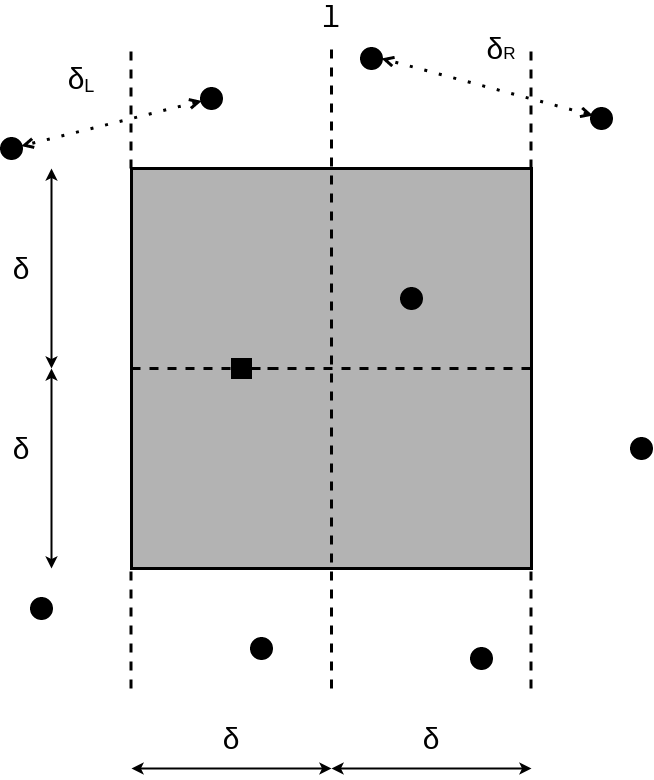
\includegraphics[width=0.5\textwidth,height=0.35\textheight]{./Combine.png}
\caption[]{The \isa{combine} step}
\label{fig:Combine}
\end{figure}
%
If \isa{p} is one of the points of the closest pair, then the distance to its closest
neighbor is strictly less than $\delta$ and we only have to check all points $q \in \mathit{set\ ps}$
that are contained within the $2\delta$ wide horizontal strip centered around the $y$-coordinate of \isa{p}.

In Section \ref{section:proving_running_time} we prove that, for each $p \in \mathit{set\ ps}$, it suffices to check
only a constant number of closest point candidates. This fact allows for an implementation of
the \isa{combine} step that runs in linear time and ultimately lets us achieve the familiar recurrence
of $T(n) = T(\lceil n/2 \rceil) + T(\lfloor n/2 \rfloor) + \mathcal{O}(n)$,
which results in the running time of $\mathcal{O}(n \log n)$.

We glossed over some implementation details to achieve this time complexity.
In Section \ref{section:proving_functional_correctness} we refine the algorithm and
in Section \ref{section:proving_running_time} we prove the $\mathcal{O}(n \log n)$ running time.


\section{Implementation and Functional Correctness Proof}
\label{section:proving_functional_correctness}

We present the implementation of the divide-and-conquer algorithm and the corresponding correctness proofs
using a bottom-up approach, starting with the \isa{combine} step. The basis for both implementation and proof is the version
presented by Cormen \emph{et al.} \cite{Introduction-to-Algorithms:2009}. But first we need to define the closest pair problem formally.

A point in the two-dimensional Euclidean plane is represented as a pair of (unbounded)
integers\footnote{We choose integers over reals because be we cannot implement
mathematical reals. See Section \ref{section:executable_code}. Alternatively we could have chosen rationals.}.
The library HOL-Analysis provides a generic distance function \isa{dist} applicable to our point definition.
The definition of this specific \isa{dist} instance corresponds to the familiar Euclidean distance measure.

The closest pair problem can be stated formally as follows: A set of points $P$ is $\mathbf{\delta}$\textbf{-sparse} iff
$\delta$ is a lower bound for the distance of all distinct pairs of points of $P$.

\begin{quote}
%
\begin{isabelle}%
sparse\ {\isasymdelta}\ P\ {\isacharequal}\ {\isacharparenleft}{\isasymforall}p\isactrlsub {\isadigit{0}}\ {\isasymin}\ P{\isachardot}\ {\isasymforall}p\isactrlsub {\isadigit{1}}\ {\isasymin}\ P{\isachardot}\ p\isactrlsub {\isadigit{0}}\ {\isasymnoteq}\ p\isactrlsub {\isadigit{1}}\ {\isasymlongrightarrow}\ {\isasymdelta}\ {\isasymle}\ dist\ p\isactrlsub {\isadigit{0}}\ p\isactrlsub {\isadigit{1}}{\isacharparenright}%
\end{isabelle}
\end{quote}
We can now state easily when two points \isa{p\isactrlsub {\isadigit{0}}} and \isa{p\isactrlsub {\isadigit{1}}} are a \textit{closest pair} of $P$: \mbox{\isa{p\isactrlsub {\isadigit{0}}\ {\isasymin}\ P}}, \isa{p\isactrlsub {\isadigit{1}}\ {\isasymin}\ P}, \isa{p\isactrlsub {\isadigit{0}}\ {\isasymnoteq}\ p\isactrlsub {\isadigit{1}}}
and (most importantly) \isa{sparse\ {\isacharparenleft}dist\ p\isactrlsub {\isadigit{0}}\ p\isactrlsub {\isadigit{1}}{\isacharparenright}\ P}.

In the following we focus on outlining the proof of the sparsity property of our implementation,
without going into the details. The additional
set membership and distinctness properties of a closest pair can be proved relatively straightforwardly
by adhering to a similar proof structure.

\subsection{The Combine Step}

The essence of the \isa{combine} step deals with the following scenario: We are given an initial pair of points
with a distance of $\delta$ and a list $\mathit{ps}$ of points, sorted in ascending order by $y$-coordinate,
that are contained in the $2\delta$ wide vertical strip centered around $l$ (see Figure \ref{fig:Combine}). Our task is to
efficiently compute a pair of points with a distance $\delta' \le \delta$ such that $\mathit{ps}$ is $\delta'$-sparse.
The recursive function \isa{find{\isacharunderscore}closest{\isacharunderscore}pair} achieves this by iterating over $\mathit{ps}$, computing
for each point its closest neighbor by calling the recursive function \textit{find\_closest} that
considers only the points within the shaded square of Figure \ref{fig:Combine}, and updating the
current pair of closest points if the newly found pair is closer together. We omit the implementation of the trivial base cases.

\begin{quote}
\isa{{\isachardoublequote}find{\isacharunderscore}closest{\isacharunderscore}pair\ {\isacharcolon}{\isacharcolon}\ point\ {\isasymtimes}\ point\ {\isasymRightarrow}\ point\ list\ {\isasymRightarrow}\ point\ {\isasymtimes}\ point{\isachardoublequote}} \vskip 0pt
\isa{find{\isacharunderscore}closest{\isacharunderscore}pair\ {\isacharparenleft}c\isactrlsub {\isadigit{0}}{\isacharcomma}\ c\isactrlsub {\isadigit{1}}{\isacharparenright}\ {\isacharparenleft}p\isactrlsub {\isadigit{0}}\ {\isacharhash}\ ps{\isacharparenright}\ {\isacharequal}\isanewline
{\isacharparenleft}\textsf{let}\ p\isactrlsub {\isadigit{1}}\ {\isacharequal}\ find{\isacharunderscore}closest\ p\isactrlsub {\isadigit{0}}\ {\isacharparenleft}dist\ c\isactrlsub {\isadigit{0}}\ c\isactrlsub {\isadigit{1}}{\isacharparenright}\ ps\isanewline
\isaindent{{\isacharparenleft}}\textsf{in}\ \textsf{if}\ dist\ c\isactrlsub {\isadigit{0}}\ c\isactrlsub {\isadigit{1}}\ {\isasymle}\ dist\ p\isactrlsub {\isadigit{0}}\ p\isactrlsub {\isadigit{1}}\ \textsf{then}\ find{\isacharunderscore}closest{\isacharunderscore}pair\ {\isacharparenleft}c\isactrlsub {\isadigit{0}}{\isacharcomma}\ c\isactrlsub {\isadigit{1}}{\isacharparenright}\ ps\isanewline
\isaindent{{\isacharparenleft}\textsf{in}\ }\textsf{else}\ find{\isacharunderscore}closest{\isacharunderscore}pair\ {\isacharparenleft}p\isactrlsub {\isadigit{0}}{\isacharcomma}\ p\isactrlsub {\isadigit{1}}{\isacharparenright}\ ps{\isacharparenright}}
\end{quote}

\begin{quote}
\isa{{\isachardoublequote}find{\isacharunderscore}closest\ {\isacharcolon}{\isacharcolon}\ point\ {\isasymRightarrow}\ real\ {\isasymRightarrow}\ point\ list\ {\isasymRightarrow}\ point{\isachardoublequote}} \vskip 0pt
\isa{find{\isacharunderscore}closest\ p\ {\isasymdelta}\ {\isacharparenleft}p\isactrlsub {\isadigit{0}}\ {\isacharhash}\ ps{\isacharparenright}\ {\isacharequal}\isanewline
{\isacharparenleft}\textsf{if}\ {\isasymdelta}\ {\isasymle}\ snd\ p\isactrlsub {\isadigit{0}}\ {\isacharminus}\ snd\ p\ \textsf{then}\ p\isactrlsub {\isadigit{0}}\isanewline
\isaindent{{\isacharparenleft}}\textsf{else}\ \textsf{let}\ p\isactrlsub {\isadigit{1}}\ {\isacharequal}\ find{\isacharunderscore}closest\ p\ {\isacharparenleft}min\ {\isasymdelta}\ {\isacharparenleft}dist\ p\ p\isactrlsub {\isadigit{0}}{\isacharparenright}{\isacharparenright}\ ps\isanewline
\isaindent{{\isacharparenleft}\textsf{else}\ }\textsf{in}\ \textsf{if}\ dist\ p\ p\isactrlsub {\isadigit{0}}\ {\isasymle}\ dist\ p\ p\isactrlsub {\isadigit{1}}\ \textsf{then}\ p\isactrlsub {\isadigit{0}}\ \textsf{else}\ p\isactrlsub {\isadigit{1}}{\isacharparenright}}
\end{quote}

There are several noteworthy aspects of this implementation. The recursive search for the closest neighbor
of a given point $p$ of \isa{find{\isacharunderscore}closest} starts at the first point spatially above $p$, continues upwards and
is stopped early at the first point whose vertical distance to $p$ is equal to or exceeds the given $\delta$. Thus the function
considers, in contrast to Figure \ref{fig:Combine}, only the upper half of the shaded square during this search.
This is sufficient for the computation of a closest pair because for each possible point $q$ preceding $p$ in
$\mathit{ps}$ we already considered the pair $(q,\,p)$, if needed, and do not have to re-check $(p,\,q)$ due to the
commutative property of our closest pair definition. Note also that $\delta$ is updated, if possible,
during the computation and consequently the search space for each point is limited to a $2\delta \times \delta'$
rectangle with $\delta' \le \delta$. Lastly we intentionally do not minimize the number of distance computations.
In Section \ref{section:executable_code} we make this optimization for the final executable code.

The following lemma captures the desired sparsity property of our implementation of the \isa{combine} step so far. It is proved by induction on the computation.

\begin{lemma} \label{lemma:find_closest_pair_dist}
\isa{sorted{\isacharunderscore}snd\ ps\ {\isasymand}\ {\isacharparenleft}p\isactrlsub {\isadigit{0}}{\isacharcomma}\ p\isactrlsub {\isadigit{1}}{\isacharparenright}\ {\isacharequal}\ find{\isacharunderscore}closest{\isacharunderscore}pair\ {\isacharparenleft}c\isactrlsub {\isadigit{0}}{\isacharcomma}\ c\isactrlsub {\isadigit{1}}{\isacharparenright}\ ps} \vskip 0pt
\isa{{\isasymLongrightarrow}\ sparse\ {\isacharparenleft}dist\ p\isactrlsub {\isadigit{0}}\ p\isactrlsub {\isadigit{1}}{\isacharparenright}\ {\isacharparenleft}set\ ps{\isacharparenright}}
\end{lemma}
where \isa{sorted{\isacharunderscore}snd\ ps} means that \isa{ps} is sorted in ascending order by $y$-coordinate.

We wrap up the \isa{combine} step by limiting our search for the closest pair to only the points contained within the
$2\delta$ wide vertical strip and choosing as argument for the initial pair of points of \textit{find\_closest\_pair}
the closest pair of the two recursive invocations of our divide-and-conquer algorithm with the smaller distance $\delta$.

\vskip 10pt
\begin{adjustwidth}{-15pt}{0pt}
\begin{quote}
\isa{{\isachardoublequote}combine\ {\isacharcolon}{\isacharcolon}\ point\ {\isasymtimes}\ point\ {\isasymRightarrow}\ point\ {\isasymtimes}\ point\ {\isasymRightarrow}\ int\ {\isasymRightarrow}\ point\ list\ {\isasymRightarrow}\ point\ {\isasymtimes}\ point{\isachardoublequote}} \vskip 0pt
\isa{combine\ {\isacharparenleft}p\isactrlsub {\isadigit{0}}\isactrlsub L{\isacharcomma}\ p\isactrlsub {\isadigit{1}}\isactrlsub L{\isacharparenright}\ {\isacharparenleft}p\isactrlsub {\isadigit{0}}\isactrlsub R{\isacharcomma}\ p\isactrlsub {\isadigit{1}}\isactrlsub R{\isacharparenright}\ l\ ps\ {\isacharequal}\isanewline
{\isacharparenleft}\textsf{let}\ {\isacharparenleft}c\isactrlsub {\isadigit{0}}{\isacharcomma}\ c\isactrlsub {\isadigit{1}}{\isacharparenright}\ {\isacharequal}\isanewline
\isaindent{{\isacharparenleft}\textsf{let}\ \ \ }\textsf{if}\ dist\ p\isactrlsub {\isadigit{0}}\isactrlsub L\ p\isactrlsub {\isadigit{1}}\isactrlsub L\ {\isacharless}\ dist\ p\isactrlsub {\isadigit{0}}\isactrlsub R\ p\isactrlsub {\isadigit{1}}\isactrlsub R\ \textsf{then}\ {\isacharparenleft}p\isactrlsub {\isadigit{0}}\isactrlsub L{\isacharcomma}\ p\isactrlsub {\isadigit{1}}\isactrlsub L{\isacharparenright}\ \textsf{else}\ {\isacharparenleft}p\isactrlsub {\isadigit{0}}\isactrlsub R{\isacharcomma}\ p\isactrlsub {\isadigit{1}}\isactrlsub R{\isacharparenright}\isanewline
\isaindent{{\isacharparenleft}}\textsf{in}\ find{\isacharunderscore}closest{\isacharunderscore}pair\ {\isacharparenleft}c\isactrlsub {\isadigit{0}}{\isacharcomma}\ c\isactrlsub {\isadigit{1}}{\isacharparenright}\isanewline
\isaindent{{\isacharparenleft}\textsf{in}\ \ }{\isacharparenleft}filter\ {\isacharparenleft}{\isasymlambda}p{\isachardot}\ dist\ p\ {\isacharparenleft}l{\isacharcomma}\ snd\ p{\isacharparenright}\ {\isacharless}\ dist\ c\isactrlsub {\isadigit{0}}\ c\isactrlsub {\isadigit{1}}{\isacharparenright}\ ps{\isacharparenright}{\isacharparenright}}
\end{quote}
\end{adjustwidth}
\vskip 10pt

Lemma \ref{lemma:set_band_filter} shows that if there exists a pair \isa{{\isacharparenleft}p\isactrlsub {\isadigit{0}}{\isacharcomma}\ p\isactrlsub {\isadigit{1}}{\isacharparenright}} of distinct points with a distance \isa{{\isacharless}\ {\isasymdelta}}, then
both its points are contained in the mentioned vertical strip, otherwise we have already found our closest pair
\isa{{\isacharparenleft}c\isactrlsub {\isadigit{0}}{\isacharcomma}\ c\isactrlsub {\isadigit{1}}{\isacharparenright}}, and the pair returned by \isa{find{\isacharunderscore}closest{\isacharunderscore}pair} is its initial argument.

\begin{lemma} \label{lemma:set_band_filter}
\isa{p\isactrlsub {\isadigit{0}}\ {\isasymin}\ set\ ps\ {\isasymand}\ p\isactrlsub {\isadigit{1}}\ {\isasymin}\ set\ ps\ {\isasymand}\ p\isactrlsub {\isadigit{0}}\ {\isasymnoteq}\ p\isactrlsub {\isadigit{1}}\ {\isasymand}\ dist\ p\isactrlsub {\isadigit{0}}\ p\isactrlsub {\isadigit{1}}\ {\isacharless}\ {\isasymdelta}\ {\isasymand}} \vskip 0pt
\isa{{\isacharparenleft}{\isasymforall}p\ {\isasymin}\ P\isactrlsub L{\isachardot}\ fst\ p\ {\isasymle}\ l{\isacharparenright}\ {\isasymand}\ sparse\ {\isasymdelta}\ P\isactrlsub L\ {\isasymand}} \vskip 0pt
\isa{{\isacharparenleft}{\isasymforall}p\ {\isasymin}\ P\isactrlsub R{\isachardot}\ l\ {\isasymle}\ fst\ p{\isacharparenright}\ {\isasymand}\ sparse\ {\isasymdelta}\ P\isactrlsub R\ {\isasymand}} \vskip 0pt
\isa{set\ ps\ {\isacharequal}\ P\isactrlsub L\ {\isasymunion}\ P\isactrlsub R\ {\isasymand}\ ps{\isacharprime}\ {\isacharequal}\ filter\ {\isacharparenleft}{\isasymlambda}p{\isachardot}\ dist\ p\ {\isacharparenleft}l\ {\isacharcomma}\ snd\ p{\isacharparenright}\ {\isacharless}\ {\isasymdelta}{\isacharparenright}\ ps} \vskip 0pt
\isa{{\isasymLongrightarrow}\ p\isactrlsub {\isadigit{0}}\ {\isasymin}\ set\ ps{\isacharprime}\ {\isasymand}\ p\isactrlsub {\isadigit{1}}\ {\isasymin}\ set\ ps{\isacharprime}}
\end{lemma}

We then can prove, additionally using Lemma \ref{lemma:find_closest_pair_dist}, that \isa{combine} computes
indeed a pair of points \isa{{\isacharparenleft}p\isactrlsub {\isadigit{0}}{\isacharcomma}\ p\isactrlsub {\isadigit{1}}{\isacharparenright}} such that our given list of points \isa{ps} is (\isa{dist\ p\isactrlsub {\isadigit{0}}\ p\isactrlsub {\isadigit{1}}})-sparse.

\begin{lemma} \label{lemma:combine_dist}
\isa{sorted{\isacharunderscore}snd\ ps\ {\isasymand}\ set\ ps\ {\isacharequal}\ P\isactrlsub L\ {\isasymunion}\ P\isactrlsub R\ {\isasymand}} \vskip 0pt
\isa{{\isacharparenleft}{\isasymforall}p\ {\isasymin}\ P\isactrlsub L{\isachardot}\ fst\ p\ {\isasymle}\ l{\isacharparenright}\ {\isasymand}\ sparse\ {\isacharparenleft}dist\ p\isactrlsub {\isadigit{0}}\isactrlsub L\ p\isactrlsub {\isadigit{1}}\isactrlsub L{\isacharparenright}\ P\isactrlsub L\ {\isasymand}} \vskip 0pt
\isa{{\isacharparenleft}{\isasymforall}p\ {\isasymin}\ P\isactrlsub R{\isachardot}\ l\ {\isasymle}\ fst\ p{\isacharparenright}\ {\isasymand}\ sparse\ {\isacharparenleft}dist\ p\isactrlsub {\isadigit{0}}\isactrlsub R\ p\isactrlsub {\isadigit{1}}\isactrlsub R{\isacharparenright}\ P\isactrlsub R\ {\isasymand}} \vskip 0pt
\isa{{\isacharparenleft}p\isactrlsub {\isadigit{0}}{\isacharcomma}\ p\isactrlsub {\isadigit{1}}{\isacharparenright}\ {\isacharequal}\ combine\ {\isacharparenleft}p\isactrlsub {\isadigit{0}}\isactrlsub L{\isacharcomma}\ p\isactrlsub {\isadigit{1}}\isactrlsub L{\isacharparenright}\ {\isacharparenleft}p\isactrlsub {\isadigit{0}}\isactrlsub R{\isacharcomma}\ p\isactrlsub {\isadigit{1}}\isactrlsub R{\isacharparenright}\ l\ ps} \vskip 0pt
\isa{{\isasymLongrightarrow}\ sparse\ {\isacharparenleft}dist\ p\isactrlsub {\isadigit{0}}\ p\isactrlsub {\isadigit{1}}{\isacharparenright}\ {\isacharparenleft}set\ ps{\isacharparenright}}
\end{lemma}

One can also show that \isa{p\isactrlsub {\isadigit{0}}} and \isa{p\isactrlsub {\isadigit{1}}} are in \isa{ps} and distinct (and thus a closest pair of \isa{set\ ps}),
if \isa{p\isactrlsub {\isadigit{0}}\isactrlsub L} (\isa{p\isactrlsub {\isadigit{0}}\isactrlsub R}) and \isa{p\isactrlsub {\isadigit{1}}\isactrlsub L} (\isa{p\isactrlsub {\isadigit{1}}\isactrlsub R}) are in \isa{P\isactrlsub L} (\isa{P\isactrlsub R}) and distinct.

\subsection{The Divide \& Conquer Algorithm} \label{subsection:dc:fc}

In Section \ref{section:closest_pair_algorithm} we glossed over some implementation detail which
is necessary to achieve to running time of $\mathcal{O}(n \log n)$. In particular
we need to partition the given list\footnote{Our implementation deals with
concrete lists in contrast to the abstract sets used in Section \ref{section:closest_pair_algorithm}.} of points $\mathit{ps}$
along a vertical line $l$ into two lists of nearly equal length during the divide step and obtain
a list $\mathit{ys}$ of the same points, sorted in ascending order by $y$-coordinate, for the \isa{combine}
step in \emph{linear} time at each level of recursion.

Cormen \emph{et al.} propose the following top-down approach: Their algorithm takes three arguments: the set
of points \isa{P} and lists \isa{xs} and \isa{ys} which contain the same set of points \isa{P} but are respectively
sorted by \isa{x} and \isa{y}-coordinate. The algorithm first splits \isa{xs} at \isa{length\ xs\ div\ {\isadigit{2}}} into two still
sorted lists \isa{xs\isactrlsub L} and \isa{xs\isactrlsub R} and chooses \isa{l} as either the \isa{x}-coordinate of the last element of \isa{xs\isactrlsub L}
or the \isa{x}-coordinate of the first element of \isa{xs\isactrlsub R}. It then constructs the sets \isa{P\isactrlsub L} and \isa{P\isactrlsub R} respectively consisting
of the points of \isa{xs\isactrlsub L} and \isa{xs\isactrlsub R}. For the recursive invocations it needs to obtain in addition lists
\isa{ys\isactrlsub L} and \isa{ys\isactrlsub R} that are still sorted by \isa{y}-coordinate and again respectively refer to the same points as
\isa{xs\isactrlsub L} and \isa{xs\isactrlsub R}. It achieves this by iterating once through \isa{ys} and checking for each point if it is
contained in \isa{P\isactrlsub L} or not, constructing \isa{ys\isactrlsub L} and \isa{ys\isactrlsub R} along the way.

But this approach requires an implementation of sets. In fact, if we want to
achieve the overall worst case running time of $\mathcal{O}(n \log n)$ it requires an implementation
of sets with linear time construction and constant time membership test, which is nontrivial, in
particular in a functional setting. To avoid sets many publications and implementations either assume
all points have unique \isa{x}-coordinates or preprocess the points by applying for example a rotation
such that the input fulfills this condition. For distinct \isa{x}-coordinates one can then compute \isa{ys\isactrlsub L}
and \isa{ys\isactrlsub R} by simply filtering \isa{ys} depending on the \isa{x}-coordinate of the points relative to \isa{l} and
eliminate the usage of sets entirely.

But there exists a third option which we have found only in Cormen \emph{et al.} where it is merely hinted at in an exercise left to the reader. The approach is the following.
Looking at the overall structure of the closest pair algorithm
we recognize that it closely resembles the structure of a standard mergesort implementation and that
we only need \isa{ys} for the \isa{combine} step \emph{after} the two recursive invocations of the algorithm.
Thus we can obtain \isa{ys} by merging `along the way' using a bottom-up approach. This is the actual code:

\begin{quote}
\isa{{\isachardoublequote}closest{\isacharunderscore}pair{\isacharunderscore}rec\ {\isacharcolon}{\isacharcolon}\ point\ list\ {\isasymRightarrow}\ point\ list\ {\isasymtimes}\ point\ {\isasymtimes}\ point{\isachardoublequote}} \vskip 0pt
\isa{closest{\isacharunderscore}pair{\isacharunderscore}rec\ xs\ {\isacharequal}\isanewline
{\isacharparenleft}\textsf{let}\ n\ {\isacharequal}\ length\ xs\isanewline
\isaindent{{\isacharparenleft}}\textsf{in}\ \textsf{if}\ n\ {\isasymle}\ {\isadigit{3}}\ \textsf{then}\ {\isacharparenleft}mergesort\ snd\ xs{\isacharcomma}\ closest{\isacharunderscore}pair{\isacharunderscore}bf\ xs{\isacharparenright}\isanewline
\isaindent{{\isacharparenleft}\textsf{in}\ }\textsf{else}\ \textsf{let}\ {\isacharparenleft}xs\isactrlsub L{\isacharcomma}\ xs\isactrlsub R{\isacharparenright}\ {\isacharequal}\ split{\isacharunderscore}at\ {\isacharparenleft}n\ div\ {\isadigit{2}}{\isacharparenright}\ xs{\isacharsemicolon}\isanewline
\isaindent{{\isacharparenleft}\textsf{in}\ \textsf{else}\ \textsf{let}\ }{\isacharparenleft}ys\isactrlsub L{\isacharcomma}\ p\isactrlsub {\isadigit{0}}\isactrlsub L{\isacharcomma}\ p\isactrlsub {\isadigit{1}}\isactrlsub L{\isacharparenright}\ {\isacharequal}\ closest{\isacharunderscore}pair{\isacharunderscore}rec\ xs\isactrlsub L{\isacharsemicolon}\isanewline
\isaindent{{\isacharparenleft}\textsf{in}\ \textsf{else}\ \textsf{let}\ }{\isacharparenleft}ys\isactrlsub R{\isacharcomma}\ p\isactrlsub {\isadigit{0}}\isactrlsub R{\isacharcomma}\ p\isactrlsub {\isadigit{1}}\isactrlsub R{\isacharparenright}\ {\isacharequal}\ closest{\isacharunderscore}pair{\isacharunderscore}rec\ xs\isactrlsub R{\isacharsemicolon}\isanewline
\isaindent{{\isacharparenleft}\textsf{in}\ \textsf{else}\ \textsf{let}\ }ys\ {\isacharequal}\ merge\ snd\ ys\isactrlsub L\ ys\isactrlsub R\isanewline
\isaindent{{\isacharparenleft}\textsf{in}\ \textsf{else}\ }\textsf{in}\ {\isacharparenleft}ys{\isacharcomma}\ combine\ {\isacharparenleft}p\isactrlsub {\isadigit{0}}\isactrlsub L{\isacharcomma}\ p\isactrlsub {\isadigit{1}}\isactrlsub L{\isacharparenright}\ {\isacharparenleft}p\isactrlsub {\isadigit{0}}\isactrlsub R{\isacharcomma}\ p\isactrlsub {\isadigit{1}}\isactrlsub R{\isacharparenright}\ {\isacharparenleft}fst\ {\isacharparenleft}hd\ xs\isactrlsub R{\isacharparenright}{\isacharparenright}\ ys{\isacharparenright}{\isacharparenright}}
\end{quote}

\begin{quote}
\isa{{\isachardoublequote}closest{\isacharunderscore}pair\ {\isacharcolon}{\isacharcolon}\ point\ list\ {\isasymRightarrow}\ point\ {\isasymtimes}\ point{\isachardoublequote}} \vskip 0pt
\isa{closest{\isacharunderscore}pair\ ps\ {\isacharequal}\isanewline
{\isacharparenleft}\textsf{let}\ {\isacharparenleft}ys{\isacharcomma}\ c\isactrlsub {\isadigit{0}}{\isacharcomma}\ c\isactrlsub {\isadigit{1}}{\isacharparenright}\ {\isacharequal}\ closest{\isacharunderscore}pair{\isacharunderscore}rec\ {\isacharparenleft}mergesort\ fst\ ps{\isacharparenright}\ \textsf{in}\ {\isacharparenleft}c\isactrlsub {\isadigit{0}}{\isacharcomma}\ c\isactrlsub {\isadigit{1}}{\isacharparenright}{\isacharparenright}}
\end{quote}

Function \isa{closest{\isacharunderscore}pair{\isacharunderscore}rec} expects a list of points \isa{xs} sorted by \isa{x}-coordinate. The
construction of \isa{xs\isactrlsub L}, \isa{xs\isactrlsub R} and \isa{l} is analogous to Cormen \emph{et al}. In the base case we then
sort \isa{xs} by \isa{y}-coordinate and compute the closest pair using the brute-force approach
(\isa{closest{\isacharunderscore}pair{\isacharunderscore}bf}). The recursive call of the algorithm on \isa{xs\isactrlsub L} returns in addition to the
closest pair of \isa{xs\isactrlsub L} the list \isa{ys\isactrlsub L}, containing all points of \isa{xs\isactrlsub L} but now sorted by \isa{y}-coordinate.
Analogously for \isa{xs\isactrlsub R} and \isa{ys\isactrlsub R}. Furthermore, we reuse function \isa{merge} from our \isa{mergesort}
implementation, which we utilize to presort the points by \isa{x}-coordinate, to obtain \isa{ys} from \isa{ys\isactrlsub L}
and \isa{ys\isactrlsub R} in linear time at each level of recursion.

Splitting of \isa{xs} is performed
by the function \isa{split{\isacharunderscore}at} via a simple linear pass over \isa{xs}. Our implementation of
\isa{mergesort} sorts a list of points depending on a given projection function, \isa{fst}
for `by \isa{x}-coordinate' and \isa{snd} for `by \isa{y}-coordinate'.

Using Lemma \ref{lemma:combine_dist}, the functional correctness proofs of our mergesort implementation
and several auxiliary lemmas proving that \textit{closest\_pair\_rec} also sorts the points by $y$-coordinate,
we arrive at the correctness proof of the desired sparsity property of the algorithm.

\begin{theorem}
\isa{{\isadigit{1}}\ {\isacharless}\ length\ xs\ {\isasymand}\ sorted{\isacharunderscore}fst\ xs\ {\isasymand}\ {\isacharparenleft}ys{\isacharcomma}\ p\isactrlsub {\isadigit{0}}{\isacharcomma}\ p\isactrlsub {\isadigit{1}}{\isacharparenright}\ {\isacharequal}\ closest{\isacharunderscore}pair{\isacharunderscore}rec\ xs} \vskip 0pt
\isa{{\isasymLongrightarrow}\ sparse\ {\isacharparenleft}dist\ p\isactrlsub {\isadigit{0}}\ p\isactrlsub {\isadigit{1}}{\isacharparenright}\ xs}
\end{theorem}

Corollary \ref{cor:closest_pair_dist} together with Theorems \ref{thm:closest_pair_set} and
\ref{thm:closest_pair_distinct} then show that the pair \isa{{\isacharparenleft}p\isactrlsub {\isadigit{0}}{\isacharcomma}\ p\isactrlsub {\isadigit{1}}{\isacharparenright}} is indeed a closest pair of \isa{ps}.

\begin{corollary} \label{cor:closest_pair_dist}
\isa{{\isadigit{1}}\ {\isacharless}\ length\ ps\ {\isasymand}\ {\isacharparenleft}p\isactrlsub {\isadigit{0}}{\isacharcomma}\ p\isactrlsub {\isadigit{1}}{\isacharparenright}\ {\isacharequal}\ closest{\isacharunderscore}pair\ ps} \vskip 0pt
\isa{{\isasymLongrightarrow}\ sparse\ {\isacharparenleft}dist\ p\isactrlsub {\isadigit{0}}\ p\isactrlsub {\isadigit{1}}{\isacharparenright}\ ps}
\end{corollary}


\begin{theorem} \label{thm:closest_pair_set}
\isa{{\isadigit{1}}\ {\isacharless}\ length\ ps\ {\isasymand}\ {\isacharparenleft}p\isactrlsub {\isadigit{0}}{\isacharcomma}\ p\isactrlsub {\isadigit{1}}{\isacharparenright}\ {\isacharequal}\ closest{\isacharunderscore}pair\ ps} \vskip 0pt
\isa{{\isasymLongrightarrow}\ p\isactrlsub {\isadigit{0}}\ {\isasymin}\ set\ ps\ {\isasymand}\ p\isactrlsub {\isadigit{1}}\ {\isasymin}\ set\ ps}
\end{theorem}

\begin{theorem} \label{thm:closest_pair_distinct}
\isa{{\isadigit{1}}\ {\isacharless}\ length\ ps\ {\isasymand}\ distinct\ ps\ {\isasymand}\ {\isacharparenleft}p\isactrlsub {\isadigit{0}}{\isacharcomma}\ p\isactrlsub {\isadigit{1}}{\isacharparenright}\ {\isacharequal}\ closest{\isacharunderscore}pair\ ps} \vskip 0pt
\isa{{\isasymLongrightarrow}\ p\isactrlsub {\isadigit{0}}\ {\isasymnoteq}\ p\isactrlsub {\isadigit{1}}}
\end{theorem}


\section{Time Complexity Proof} \label{section:proving_running_time}

To formally verify the running time we follow the approach in \cite{Nipkow-APLAS17}.
For each function \isa{f} we define a function \isa{t{\isacharunderscore}f} that takes the same arguments as
\isa{f} but computes the number of function calls the computation of \isa{f} needs, the `time'.
Function \isa{t{\isacharunderscore}f} follows the same recursion structure as \isa{f} and can be seen as an
abstract interpretation of \isa{f}. To ensure the absence of errors we derive \isa{f} and
\isa{t{\isacharunderscore}f} from a monadic function that computes both the value and the time but for simplicity of
presentation we present only \isa{f} and \isa{t{\isacharunderscore}f}. We also simplify matters a bit: we count
only expensive operations where the running time increases with the size of the input; in particular
we assume constant time arithmetic and ignore small additive constants. Due to reasons of space we
only show one example of such a `timing' function, \isa{t{\isacharunderscore}find{\isacharunderscore}closest}, which is crucial to our
time complexity proof.

\begin{quote}
\isa{{\isachardoublequote}t{\isacharunderscore}find{\isacharunderscore}closest\ {\isacharcolon}{\isacharcolon}\ point\ {\isasymRightarrow}\ real\ {\isasymRightarrow}\ point\ list\ {\isasymRightarrow}\ nat{\isachardoublequote}} \vskip 0pt
\isa{t{\isacharunderscore}find{\isacharunderscore}closest\ p\ {\isasymdelta}\ {\isacharbrackleft}{\isacharbrackright}\ {\isacharequal}\ {\isadigit{0}}} \vskip 0pt
\isa{t{\isacharunderscore}find{\isacharunderscore}closest\ p\ {\isasymdelta}\ {\isacharbrackleft}p\isactrlsub {\isadigit{0}}{\isacharbrackright}\ {\isacharequal}\ {\isadigit{1}}} \vskip 0pt
\isa{t{\isacharunderscore}find{\isacharunderscore}closest\ p\ {\isasymdelta}\ {\isacharparenleft}p\isactrlsub {\isadigit{0}}\ {\isacharhash}\ ps{\isacharparenright}\ {\isacharequal}\ {\isadigit{1}}\ {\isacharplus}} \vskip 0pt
\isa{{\isacharparenleft}\textsf{if}\ {\isasymdelta}\ {\isasymle}\ snd\ p\isactrlsub {\isadigit{0}}\ {\isacharminus}\ snd\ p\ \textsf{then}\ {\isadigit{0}}} \vskip 0pt
\ \isa{\textsf{else}\ \textsf{let}\ p\isactrlsub {\isadigit{1}}\ {\isacharequal}\ find{\isacharunderscore}closest\ p\ {\isacharparenleft}min\ {\isasymdelta}\ {\isacharparenleft}dist\ p\ p\isactrlsub {\isadigit{0}}{\isacharparenright}{\isacharparenright}\ ps} \vskip 0pt
\ \qquad\isa{\textsf{in}\ t{\isacharunderscore}find{\isacharunderscore}closest\ p\ {\isacharparenleft}min\ {\isasymdelta}\ {\isacharparenleft}dist\ p\ p\isactrlsub {\isadigit{0}}{\isacharparenright}{\isacharparenright}\ ps\ {\isacharplus}} \vskip 0pt
\ \quad\qquad\isa{{\isacharparenleft}\textsf{if}\ dist\ p\ p\isactrlsub {\isadigit{0}}\ {\isasymle}\ dist\ p\ p\isactrlsub {\isadigit{1}}\ \textsf{then}\ {\isadigit{0}}\ \textsf{else}\ {\isadigit{0}}{\isacharparenright}{\isacharparenright}}
\end{quote}
%TODO less about base cases?
We set the time to execute \isa{dist} computations to \isa{{\isadigit{0}}} since it is a combination
of cheap operations. For the base cases of recursive functions
we fix the computation time to be equivalent to the size of the input. This choice of constants is arbitrary and has no
impact on the overall running time analysis but leads in general to `cleaner' arithmetic bounds.
%Note that it might be of interest to define a similar abstract interpretation to count the number of
%\isa{dist} computations of the algorithm and compare different implementation approaches with
%regard to this number. Since we choose not to minimize the number of \isa{dist} computations,
%except for the final executable code in Section \ref{section:executable_code}, we omit such an analysis.

\subsection{Time Analysis of the Combine Step}

In Section \ref{section:closest_pair_algorithm} we claimed that the running time of the algorithm is
captured by the recurrence \isa{T{\isacharparenleft}n{\isacharparenright}\ {\isacharequal}\ T{\isacharparenleft}{\isasymlceil}n{\isacharslash}{\isadigit{2}}{\isasymrceil}{\isacharparenright}\ {\isacharplus}\ T{\isacharparenleft}{\isasymlfloor}n{\isacharslash}{\isadigit{2}}{\isasymrfloor}{\isacharparenright}\ {\isacharplus}\ O{\isacharparenleft}n{\isacharparenright}},
where \isa{n} is the length of the given list of points. This claim implies an at most linear overhead
at each level of recursion. Splitting of the list \isa{xs}, merging \isa{ys\isactrlsub L} and \isa{ys\isactrlsub R} and
the filtering operation of the \isa{combine} step run in linear time. But it is non-trivial that the
function \isa{find{\isacharunderscore}closest{\isacharunderscore}pair}, central to the \isa{combine} step, also exhibits a linear
time complexity. It is applied to an argument list of, in the worst case, length \isa{n}, iterates
once through the list and calls \isa{find{\isacharunderscore}closest} for each element. Consequently our proof obligation
is the constant running time of \isa{find{\isacharunderscore}closest} or, considering our timing function, that there exists
some constant \isa{c} such that \isa{t{\isacharunderscore}find{\isacharunderscore}closest\ p\ {\isasymdelta}\ ps\ {\isasymle}\ c} holds in the context of the \isa{combine} step.

Looking at the definition of \isa{find{\isacharunderscore}closest} we see that the function terminates as soon as
it encounters the first point within the given list \isa{ps} that does not fulfill the predicate
(\isa{{\isasymlambda}q{\isachardot}\ {\isasymdelta}\ {\isasymle}\ snd\ q\ {\isacharminus}\ snd\ p}), the point \isa{p} being an argument to \isa{find{\isacharunderscore}closest},
or if \isa{ps} is a list of length \isa{{\isasymle}{\isadigit{1}}}. The corresponding timing function \isa{t{\isacharunderscore}find{\isacharunderscore}closest}
computes the number of recursive function calls, which is, in this case, synonymous with the number of examined points.
For our time complexity proof it suffices to show the following bound on the result of  \isa{t{\isacharunderscore}find{\isacharunderscore}closest}.
The proof is by induction on the computation of \isa{t{\isacharunderscore}find{\isacharunderscore}closest}. The function \isa{count\ f} is
an abbreviation for \isa{length\ {\isasymcirc}\ filter\ f}.

\begin{lemma}
\isa{t{\isacharunderscore}find{\isacharunderscore}closest\ p\ {\isasymdelta}\ ps\ {\isasymle}\ {\isadigit{1}}\ {\isacharplus}\ count\ {\isacharparenleft}{\isasymlambda}q{\isachardot}\ snd\ q\ {\isacharminus}\ snd\ p\ {\isasymle}\ {\isasymdelta}{\isacharparenright}\ ps}
\end{lemma}

Therefore we need to prove that the term  \isa{count\ {\isacharparenleft}{\isasymlambda}q{\isachardot}\ snd\ q\ {\isacharminus}\ snd\ p\ {\isasymle}\ {\isasymdelta}{\isacharparenright}\ ps} does not depend
on the length of \isa{ps}. Looking back at Figure \ref{fig:Combine}, the square point representing \isa{p},
we can assume that the list \isa{p\ {\isacharhash}\ ps} is distinct and sorted in ascending order by \isa{y}-coordinate.
From the precomputing effort of the \isa{combine} step we know that its points are contained
within the \isa{{\isadigit{2}}{\isasymdelta}} wide vertical strip centered around \isa{l} and can be split into two sets \isa{P\isactrlsub L}
(\isa{P\isactrlsub R}) consisting of all points which lie to the left (right) of or on the line \isa{l}.
Due to the two recursive invocations of the algorithm during the conquer step we can additionally assume
that both \isa{P\isactrlsub L} and \isa{P\isactrlsub R} are \isa{{\isasymdelta}}-sparse, suggesting the following lemma which implies
\isa{t{\isacharunderscore}find{\isacharunderscore}closest\ p\ {\isasymdelta}\ ps\ {\isasymle}\ {\isadigit{8}}} and thus the constant running time of \isa{find{\isacharunderscore}closest}.

\begin{lemma} \label{lemma:core_argument}
\isa{distinct\ {\isacharparenleft}p\ {\isacharhash}\ ps{\isacharparenright}\ {\isasymand}\ sorted{\isacharunderscore}snd\ {\isacharparenleft}p\ {\isacharhash}\ ps{\isacharparenright}\ {\isasymand}\ {\isadigit{0}}\ {\isasymle}\ {\isasymdelta}\ {\isasymand}} \vskip 0pt
\isa{{\isacharparenleft}{\isasymforall}q\ {\isasymin}\ set\ {\isacharparenleft}p\ {\isacharhash}\ ps{\isacharparenright}{\isachardot}\ l\ {\isacharminus}\ {\isasymdelta}\ {\isacharless}\ fst\ q\ {\isasymand}\ fst\ q\ {\isacharless}\ l\ {\isacharplus}\ {\isasymdelta}{\isacharparenright}\ {\isasymand}} \vskip 0pt
\isa{set\ {\isacharparenleft}p\ {\isacharhash}\ ps{\isacharparenright}\ {\isacharequal}\ P\isactrlsub L\ {\isasymunion}\ P\isactrlsub R\ {\isasymand}} \vskip 0pt
\isa{{\isacharparenleft}{\isasymforall}q\ {\isasymin}\ P\isactrlsub L\ {\isachardot}\ fst\ q\ {\isasymle}\ l{\isacharparenright}\ {\isasymand}\ sparse\ {\isasymdelta}\ P\isactrlsub L\ {\isasymand}} \vskip 0pt
\isa{{\isacharparenleft}{\isasymforall}q\ {\isasymin}\ P\isactrlsub R\ {\isachardot}\ l\ {\isasymle}\ fst\ q{\isacharparenright}\ {\isasymand}\ sparse\ {\isasymdelta}\ P\isactrlsub R} \vskip 0pt
\isa{{\isasymLongrightarrow}} \isa{count\ {\isacharparenleft}{\isasymlambda}q{\isachardot}\ snd\ q\ {\isacharminus}\ snd\ p\ {\isasymle}\ {\isasymdelta}{\isacharparenright}\ ps\ {\isasymle}\ {\isadigit{7}}}
\end{lemma}
\begin{proof}
The library HOL-Analysis defines some basic geometric building blocks needed for the proof. A \textit{closed box}
describes points contained within rectangular shapes in Euclidean space. For our purposes the planar definition is sufficient.

\begin{quote}
%
\begin{isabelle}%
cbox\ {\isacharparenleft}x\isactrlsub {\isadigit{0}}{\isacharcomma}\ y\isactrlsub {\isadigit{0}}{\isacharparenright}\ {\isacharparenleft}x\isactrlsub {\isadigit{1}}{\isacharcomma}\ y\isactrlsub {\isadigit{1}}{\isacharparenright}\ {\isacharequal}\ {\isacharbraceleft}{\isacharparenleft}x{\isacharcomma}\ y{\isacharparenright}\ {\isacharbar}\ x\isactrlsub {\isadigit{0}}\ {\isasymle}\ x\ {\isasymand}\ x\ {\isasymle}\ x\isactrlsub {\isadigit{1}}\ {\isasymand}\ y\isactrlsub {\isadigit{0}}\ {\isasymle}\ y\ {\isasymand}\ y\ {\isasymle}\ y\isactrlsub {\isadigit{1}}{\isacharbraceright}%
\end{isabelle}
\end{quote}

The box is `closed' since it includes points located on the border of the box. We then introduce
some useful abbreviations:

\begin{itemize}
\setlength{\itemsep}{1pt}
\setlength{\parskip}{0pt}
\setlength{\parsep}{0pt}
\item The rectangle \isa{R} is the upper half of the shaded square of Figure \ref{fig:Combine}: \\
      \isa{R\ {\isacharequal}\ cbox\ {\isacharparenleft}l\ {\isacharminus}\ {\isasymdelta}{\isacharcomma}\ snd\ p{\isacharparenright}\ {\isacharparenleft}l\ {\isacharplus}\ {\isasymdelta}{\isacharcomma}\ snd\ p\ {\isacharplus}\ {\isasymdelta}{\isacharparenright}}
\item The set \isa{R\isactrlsub p\isactrlsub s} consists of all points of \isa{p\ {\isacharhash}\ ps} that are encompassed by \isa{R}: \\
      \isa{R\isactrlsub p\isactrlsub s\ {\isacharequal}\ R\ {\isasyminter}\ set\ {\isacharparenleft}p\ {\isacharhash}\ ps{\isacharparenright}}
\item The squares \isa{S\isactrlsub L} and \isa{S\isactrlsub R} denote the left and right halves of \isa{R}: \\
      \isa{S\isactrlsub L\ {\isacharequal}\ cbox\ {\isacharparenleft}l\ {\isacharminus}\ {\isasymdelta}{\isacharcomma}\ snd\ p{\isacharparenright}\ {\isacharparenleft}l{\isacharcomma}\ snd\ p\ {\isacharplus}\ {\isasymdelta}{\isacharparenright}} \\
      \isa{S\isactrlsub R\ {\isacharequal}\ cbox\ {\isacharparenleft}l{\isacharcomma}\ snd\ p{\isacharparenright}\ {\isacharparenleft}l\ {\isacharplus}\ {\isasymdelta}{\isacharcomma}\ snd\ p\ {\isacharplus}\ {\isasymdelta}{\isacharparenright}}
\item The set \isa{S\isactrlsub P\isactrlsub L} holds all points of \isa{P\isactrlsub L} that are contained within the square \isa{S\isactrlsub L}. The definition
      of \isa{S\isactrlsub P\isactrlsub R} is analogous: \\
      \isa{S\isactrlsub P\isactrlsub L\ {\isacharequal}\ P\isactrlsub L\ {\isasyminter}\ S\isactrlsub L}, \isa{S\isactrlsub P\isactrlsub R\ {\isacharequal}\ P\isactrlsub R\ {\isasyminter}\ S\isactrlsub R}
\end{itemize}

Let additionally \isa{ps\isactrlsub f} abbreviate the term \isa{filter\ {\isacharparenleft}{\isasymlambda}q{\isachardot}\ snd\ q\ {\isacharminus}\ snd\ p\ {\isasymle}\ {\isasymdelta}{\isacharparenright}\ ps}.
First we prove \isa{length\ {\isacharparenleft}p\ {\isacharhash}\ ps\isactrlsub f{\isacharparenright}\ {\isasymle}\ {\isacharbar}R\isactrlsub p\isactrlsub s{\isacharbar}}: Let \isa{q} denote an arbitrary point of \mbox{\isa{p\ {\isacharhash}\ ps\isactrlsub f}}. We know
\isa{snd\ p\ {\isasymle}\ snd\ q} because the list \isa{p\ {\isacharhash}\ ps} and therefore \mbox{\isa{p\ {\isacharhash}\ ps\isactrlsub f}} is sorted in ascending order by \isa{y}-coordinate and
\mbox{\isa{snd\ q\ {\isasymle}\ snd\ p\ {\isacharplus}\ {\isasymdelta}}} due to the filter predicate (\isa{{\isasymlambda}q{\isachardot}\ snd\ q\ {\isacharminus}\ snd\ p\ {\isasymle}\ {\isasymdelta}}).
Using the additional facts \isa{l\ {\isacharminus}\ {\isasymdelta}\ {\isasymle}\ fst\ q} and \isa{fst\ q\ {\isasymle}\ l\ {\isacharplus}\ {\isasymdelta}} (derived from our assumption
that all points of \isa{p\ {\isacharhash}\ ps} are contained within the \isa{{\isadigit{2}}{\isasymdelta}} strip)
and the definitions of \isa{R\isactrlsub p\isactrlsub s}, \isa{R} and \isa{cbox} we know \isa{q\ {\isasymin}\ R\isactrlsub p\isactrlsub s} and thus \isa{set\ {\isacharparenleft}p\ {\isacharhash}\ ps\isactrlsub f{\isacharparenright}\ {\isasymsubseteq}\ R\isactrlsub p\isactrlsub s}.
Since the list \isa{p\ {\isacharhash}\ ps\isactrlsub f} maintains the distinctness property of \isa{p\ {\isacharhash}\ ps} we additionally have
\mbox{\isa{length\ {\isacharparenleft}p\ {\isacharhash}\ ps\isactrlsub f{\isacharparenright}\ {\isacharequal}\ {\isacharbar}set\ {\isacharparenleft}p\ {\isacharhash}\ ps\isactrlsub f{\isacharparenright}{\isacharbar}}}. Our intermediate goal immediately follows because
\isa{{\isacharbar}set\ {\isacharparenleft}p\ {\isacharhash}\ ps\isactrlsub f{\isacharparenright}{\isacharbar}\ {\isasymle}\ {\isacharbar}R\isactrlsub p\isactrlsub s{\isacharbar}} holds for the finite set \isa{R\isactrlsub p\isactrlsub s}.

But how many points can there be in \isa{R\isactrlsub p\isactrlsub s}? Lets first try to determine an upper bound for the number of points of \isa{S\isactrlsub P\isactrlsub L}.
All its points are contained within the square \isa{S\isactrlsub L} whose side length is \isa{{\isasymdelta}}. Moreover, since \isa{P\isactrlsub L} is \isa{{\isasymdelta}}-sparse and
\mbox{\isa{S\isactrlsub P\isactrlsub L\ {\isasymsubseteq}\ P\isactrlsub L}}, \isa{S\isactrlsub P\isactrlsub L} is also \isa{{\isasymdelta}}-sparse, or the distance between each distinct pair of points of \isa{S\isactrlsub P\isactrlsub L} is at least \isa{{\isasymdelta}}.
Therefore the cardinality of \isa{S\isactrlsub P\isactrlsub L} is bounded by the number of points we can maximally fit into \isa{S\isactrlsub L}, maintaining
a pairwise minimum distance of \isa{{\isasymdelta}}. As the left-hand side of Figure \ref{fig:core_arguments} depicts, we can arrange at most four points
adhering to these restrictions, and consequently have \isa{{\isacharbar}S\isactrlsub P\isactrlsub L{\isacharbar}\ {\isasymle}\ {\isadigit{4}}}. An analogous argument holds for
the number of points of \isa{S\isactrlsub P\isactrlsub R}. Furthermore we know \isa{R\isactrlsub p\isactrlsub s\ {\isacharequal}\ S\isactrlsub P\isactrlsub L\ {\isasymunion}\ S\isactrlsub P\isactrlsub R} due to our assumption
\isa{set\ {\isacharparenleft}p\ {\isacharhash}\ ps{\isacharparenright}\ {\isacharequal}\ P\isactrlsub L\ {\isasymunion}\ P\isactrlsub R} and the fact \isa{R\ {\isacharequal}\ S\isactrlsub L\ {\isasymunion}\ S\isactrlsub R} and can conclude \isa{{\isacharbar}R\isactrlsub p\isactrlsub s{\isacharbar}\ {\isasymle}\ {\isadigit{8}}}.
Our original statement then follows from \isa{length\ {\isacharparenleft}p\ {\isacharhash}\ ps\isactrlsub f{\isacharparenright}\ {\isasymle}\ {\isacharbar}R\isactrlsub p\isactrlsub s{\isacharbar}}.
\qed
\end{proof}
%
\begin{figure}[htpb]
\centering
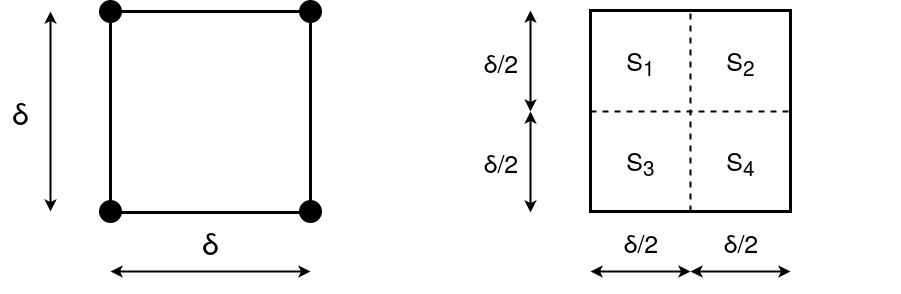
\includegraphics[width=0.75\textwidth]{./Core_Arguments.png}
\caption[]{Core Argument.}
\label{fig:core_arguments}
\end{figure}
%
Note that the intermediate proof for the bound on \isa{{\isacharbar}R\isactrlsub p\isactrlsub s{\isacharbar}} relies on basic human geometric intuition.
Indeed Cormen \emph{et al.} \cite{Introduction-to-Algorithms:2009} and most of the proofs in the literature do.
But for a formal proof we have to be rigorous. First we show two auxiliary lemmas: The maximum distance
between two points in a square \isa{S} with side length \isa{{\isasymdelta}} is less than or equal to $\sqrt{2}\delta$.

\begin{lemma} \label{lemma:max_dist_square}
\isa{p\isactrlsub {\isadigit{0}}\ {\isacharequal}\ {\isacharparenleft}x{\isacharcomma}\ y{\isacharparenright}\ {\isasymand}\ p\isactrlsub {\isadigit{1}}\ {\isacharequal}\ {\isacharparenleft}x\ {\isacharplus}\ {\isasymdelta}{\isacharcomma}\ y\ {\isacharplus}\ {\isasymdelta}{\isacharparenright}\ {\isasymand}\ {\isadigit{0}}\ {\isasymle}\ {\isasymdelta}\ {\isasymand}} \vskip 0pt
\isa{{\isacharparenleft}x\isactrlsub {\isadigit{0}}{\isacharcomma}\ y\isactrlsub {\isadigit{0}}{\isacharparenright}\ {\isasymin}\ cbox\ p\isactrlsub {\isadigit{0}}\ p\isactrlsub {\isadigit{1}}\ {\isasymand}\ {\isacharparenleft}x\isactrlsub {\isadigit{1}}{\isacharcomma}\ y\isactrlsub {\isadigit{1}}{\isacharparenright}\ {\isasymin}\ cbox\ p\isactrlsub {\isadigit{0}}\ p\isactrlsub {\isadigit{1}}} \vskip 0pt
\isa{{\isasymLongrightarrow}\ dist\ {\isacharparenleft}x\isactrlsub {\isadigit{0}}{\isacharcomma}\ y\isactrlsub {\isadigit{0}}{\isacharparenright}\ {\isacharparenleft}x\isactrlsub {\isadigit{1}}{\isacharcomma}\ y\isactrlsub {\isadigit{1}}{\isacharparenright}\ {\isasymle}\ $\sqrt{2}$\ {\isacharasterisk}\ {\isasymdelta}}
\end{lemma}

The proof is straightforward. Both points are contained within the square \isa{S}, the difference between
their \isa{x} and \isa{y} coordinates is hence bounded by \isa{{\isasymdelta}} and we finish the proof using the definition of the Euclidean
distance. Below we employ the following variation of the \textit{pigeonhole} principle:

\begin{lemma} \label{lemma:pigeonhole}
\isa{finite\ B\ {\isasymand}\ A\ {\isasymsubseteq}\ {\isasymUnion}B\ {\isasymand}} \isa{{\isacharbar}B{\isacharbar}\ {\isacharless}\ {\isacharbar}A{\isacharbar}} \vskip 0pt
\isa{{\isasymLongrightarrow}\ {\isasymexists}x\ {\isasymin}\ A{\isachardot}\ {\isasymexists}y\ {\isasymin}\ A{\isachardot}\ {\isasymexists}S\ {\isasymin}\ B{\isachardot}\ x\ {\isasymnoteq}\ y\ {\isasymand}\ x\ {\isasymin}\ S\ {\isasymand}\ y\ {\isasymin}\ S}
\end{lemma}

%The proof is by contradiction using the following chain of inequalities:
%$$\lvert B \rvert < \lvert A \cap \bigcup B \rvert \le \sum S \in B.\ \lvert A \cap S \rvert \le \lvert B \rvert$$
%The first inequality holds using our assumptions \isa{A\ {\isasymsubseteq}\ {\isasymUnion}\ B} and \isa{{\isacharbar}B{\isacharbar}\ {\isacharless}\ {\isacharbar}A{\isacharbar}}.
%The second inequality can be shown by induction over the cardinality of \isa{B}. Let then \isa{x} and \isa{y} denote
%arbitrary elements of \isa{A} and \isa{S} be an arbitrary set of \isa{B}. Suppose, for the sake of contradiction,
%either \isa{x\ {\isacharequal}\ y}, or \isa{x\ {\isasymnotin}\ S}, or \isa{y\ {\isasymnotin}\ S} then \isa{{\isacharbar}A\ {\isasyminter}\ S{\isacharbar}\ {\isasymle}\ {\isadigit{1}}} must hold. The proof
%is again by contradiction: Suppose \isa{{\isadigit{1}}\ {\isacharless}\ {\isacharbar}A\ {\isasyminter}\ S{\isacharbar}}, then there exists a distinct pair of elements
%which are both element of \isa{S}. A contradiction to our previous assumptions for \isa{x} and \isa{y}. Thus the third inequality
%is correct and we have shown \isa{{\isacharbar}B{\isacharbar}\ {\isacharless}\ {\isacharbar}B{\isacharbar}}, a contradiction.

Finally we replace human intuition with formal proof:

\begin{lemma}
\isa{{\isacharparenleft}{\isasymforall}p\ {\isasymin}\ P{\isachardot}\ p\ {\isasymin}\ cbox\ {\isacharparenleft}x{\isacharcomma}\ y{\isacharparenright}\ {\isacharparenleft}x\ {\isacharplus}\ {\isasymdelta}{\isacharcomma}\ y\ {\isacharplus}\ {\isasymdelta}{\isacharparenright}{\isacharparenright}\ {\isasymand}\ sparse\ {\isasymdelta}\ P\ {\isasymand}\ {\isadigit{0}}\ {\isasymle}\ {\isasymdelta}} \vskip 0pt
\isa{{\isasymLongrightarrow}} \isa{{\isacharbar}P{\isacharbar}\ {\isasymle}\ {\isadigit{4}}}
\end{lemma}
\begin{proof}
Let \isa{S} denote the square with a side length of \isa{{\isasymdelta}} and suppose, for the sake of contradiction, that \isa{{\isadigit{4}}\ {\isacharless}\ {\isacharbar}P{\isacharbar}}.
Then \isa{S} can be split into the four congruent squares \isa{S\isactrlsub {\isadigit{1}}{\isacharcomma}\ S\isactrlsub {\isadigit{2}}{\isacharcomma}\ S\isactrlsub {\isadigit{3}}{\isacharcomma}\ S\isactrlsub {\isadigit{4}}} along the common point
\isa{{\isacharparenleft}x\ {\isacharplus}\ {\isasymdelta}{\isacharslash}{\isadigit{2}}{\isacharcomma}\ y\ {\isacharplus}\ {\isasymdelta}{\isacharslash}{\isadigit{2}}{\isacharparenright}} as depicted by the right-hand side of Figure \ref{fig:core_arguments}.
Since all points of \isa{P} are contained within \isa{S} and \isa{S\ {\isacharequal}\ {\isasymUnion}\ {\isacharbraceleft}S\isactrlsub {\isadigit{1}}{\isacharcomma}\ S\isactrlsub {\isadigit{2}}{\isacharcomma}\ S\isactrlsub {\isadigit{3}}{\isacharcomma}\ S\isactrlsub {\isadigit{4}}{\isacharbraceright}} we have \isa{P\ {\isasymsubseteq}\ {\isasymUnion}\ {\isacharbraceleft}S\isactrlsub {\isadigit{1}}{\isacharcomma}\ S\isactrlsub {\isadigit{2}}{\isacharcomma}\ S\isactrlsub {\isadigit{3}}{\isacharcomma}\ S\isactrlsub {\isadigit{4}}{\isacharbraceright}}.
Using Lemma \ref{lemma:pigeonhole} and our assumption  \isa{{\isadigit{4}}\ {\isacharless}\ {\isacharbar}P{\isacharbar}} we know there exists a square
\mbox{\isa{S\isactrlsub i\ {\isasymin}\ {\isacharbraceleft}S\isactrlsub {\isadigit{1}}{\isacharcomma}\ S\isactrlsub {\isadigit{2}}{\isacharcomma}\ S\isactrlsub {\isadigit{3}}{\isacharcomma}\ S\isactrlsub {\isadigit{4}}{\isacharbraceright}}} and a pair of distinct points \isa{p\isactrlsub {\isadigit{0}}\ {\isasymin}\ S\isactrlsub i} and \isa{p\isactrlsub {\isadigit{1}}\ {\isasymin}\ S\isactrlsub i}.
Lemma \ref{lemma:max_dist_square} and the fact that all four sub-squares have the same side length \isa{{\isasymdelta}\ {\isacharslash}\ {\isadigit{2}}}
shows that the distance between \isa{p\isactrlsub {\isadigit{0}}} and \isa{p\isactrlsub {\isadigit{1}}} must be less than or equal to \isa{$\sqrt{2}$\ {\isacharslash}\ {\isadigit{2}}\ {\isacharasterisk}\ {\isasymdelta}} and hence
strictly less than \isa{{\isasymdelta}}. But we also know that \isa{{\isasymdelta}} is a lower bound for this distance because \isa{p\isactrlsub {\isadigit{0}}\ {\isasymin}\ P},
\isa{p\isactrlsub {\isadigit{0}}\ {\isasymin}\ P}, \isa{p\isactrlsub {\isadigit{0}}\ {\isasymnoteq}\ p\isactrlsub {\isadigit{1}}} and our premise that \isa{P} is \isa{{\isasymdelta}}-sparse, a contradiction.\qed
\end{proof}

\subsection{Time Analysis of the Divide \& Conquer Algorithm}

In summary, the time to evaluate \isa{find{\isacharunderscore}closest\ p\ {\isasymdelta}\ ps} is constant in the context of the \isa{combine} step
and thus evaluating \isa{find{\isacharunderscore}closest{\isacharunderscore}pair\ {\isacharparenleft}p\isactrlsub {\isadigit{0}}{\isacharcomma}\ p\isactrlsub {\isadigit{1}}{\isacharparenright}\ ps} as well as \isa{combine\ {\isacharparenleft}p\isactrlsub {\isadigit{0}}\isactrlsub L{\isacharcomma}\ p\isactrlsub {\isadigit{1}}\isactrlsub L{\isacharparenright}\ {\isacharparenleft}p\isactrlsub {\isadigit{0}}\isactrlsub R{\isacharcomma}\ p\isactrlsub {\isadigit{1}}\isactrlsub R{\isacharparenright}\ l\ ps}
takes time linear in \isa{length\ ps}.

Next we turn our attention to the timing of \isa{closest{\isacharunderscore}pair{\isacharunderscore}rec}
and derive (but do not show) the corresponding function \isa{t{\isacharunderscore}closest{\isacharunderscore}pair{\isacharunderscore}rec}.
At this point we could prove a concrete bound on \isa{t{\isacharunderscore}closest{\isacharunderscore}pair{\isacharunderscore}rec}.
But since we are dealing with a divide-and-conquer algorithm we should, in theory, be able to determine its
running time using the `master theorem' \cite{Introduction-to-Algorithms:2009}. This is, in practice, also
possible in Isabelle/HOL. Eberl \cite{eberl_akra_bazzi} has formalized the Akra-Bazzi theorem \cite{Akra1998},
a generalization of the master theorem. Using this formalization we can derive the running time of
our divide-and-conquer algorithm without a direct proof for \isa{t{\isacharunderscore}closest{\isacharunderscore}pair{\isacharunderscore}rec}. First
we capture the essence of \isa{t{\isacharunderscore}closest{\isacharunderscore}pair{\isacharunderscore}rec} as a recurrence on natural numbers
representing the length of the list argument of \isa{{\isacharparenleft}t{\isacharunderscore}{\isacharparenright}}\isa{closest{\isacharunderscore}pair{\isacharunderscore}rec}:
%
\begin{quote}
\isa{closest{\isacharunderscore}pair{\isacharunderscore}recurrence\ {\isacharcolon}{\isacharcolon}\ nat\ {\isasymRightarrow}\ real} \vskip 0pt
\isa{closest{\isacharunderscore}pair{\isacharunderscore}recurrence\ n\ {\isacharequal}\isanewline
{\isacharparenleft}\textsf{if}\ n\ {\isasymle}\ {\isadigit{3}}\ \textsf{then}\ n\ {\isacharplus}\ mergesort{\isacharunderscore}recurrence\ n\ {\isacharplus}\ n\ {\isacharasterisk}\ n\isanewline
\isaindent{{\isacharparenleft}}\textsf{else}\ {\isadigit{1}}{\isadigit{3}}\ {\isacharasterisk}\ n\ {\isacharplus}\ closest{\isacharunderscore}pair{\isacharunderscore}recurrence\ {\isasymlfloor}n\ {\isacharslash}\ {\isadigit{2}}{\isasymrfloor}\ {\isacharplus}\isanewline
\isaindent{{\isacharparenleft}\textsf{else}\ }closest{\isacharunderscore}pair{\isacharunderscore}recurrence\ {\isasymlceil}n\ {\isacharslash}\ {\isadigit{2}}{\isasymrceil}{\isacharparenright}}
\end{quote}

The time complexity of this recurrence is proved completely automatically:

\begin{lemma} \label{lemma:closest_pair_recurrence}
\isa{closest{\isacharunderscore}pair{\isacharunderscore}recurrence\ {\isasymin}\ {\isasymTheta}{\isacharparenleft}{\isasymlambda}n{\isachardot}\ n\ {\isacharasterisk}\ $\ln$\ n{\isacharparenright}}
\end{lemma}

Next we need to connect this bound with our timing function. Lemma \ref{lemma:bigo_measure_trans} below
expresses a procedure for deriving complexity properties of the form

\begin{quote}
\isa{t\ {\isasymin}\ O{\isacharbrackleft}m\ going{\isacharunderscore}to\ at{\isacharunderscore}top\ within\ A{\isacharbrackright}{\isacharparenleft}f\ {\isasymcirc}\ m{\isacharparenright}}
\end{quote}

where \isa{t} is a timing function on the data domain, in our case lists. The function \isa{m} is a measure
on that data domain, \isa{r} is a recurrence or any other function of type \isa{nat\ {\isasymRightarrow}\ real} and \isa{A}
is the set of valid inputs. The term `\isa{m\ going{\isacharunderscore}to\ at{\isacharunderscore}top\ within\ A}' should be read as
`if the measured size of valid inputs is sufficiently large' and utilizes Eberls formalization of
Landau Notation \cite{eberl19issac} and the ``filter'' machinery of asymptotics in Isabelle/HOL
\cite{filter}. For readability we omit stating the filter and \isa{m} explicitly in the following and
just state the  conditions required of the input \isa{A}. The measure \isa{m} always corresponds to the
\isa{length} function.

\begin{lemma} \label{lemma:bigo_measure_trans}
\isa{{\isacharparenleft}{\isasymforall}x\ {\isasymin}\ A{\isachardot}\ t\ x\ {\isasymle}\ {\isacharparenleft}r\ {\isasymcirc}\ m{\isacharparenright}\ x{\isacharparenright}\ {\isasymand}\ r\ {\isasymin}\ O{\isacharparenleft}f{\isacharparenright}\ {\isasymand}\ {\isacharparenleft}{\isasymforall}x\ {\isasymin}\ A{\isachardot}\ {\isadigit{0}}\ {\isasymle}\ t\ x{\isacharparenright}} \vskip 0pt
\isa{{\isasymLongrightarrow}\ t\ {\isasymin}\ O{\isacharbrackleft}m\ going{\isacharunderscore}to\ at{\isacharunderscore}top\ within\ A{\isacharbrackright}{\isacharparenleft}f\ {\isasymcirc}\ m{\isacharparenright}}
\end{lemma}

\begin{lemma}\label{lemma:recurrence}
\isa{distinct\ ps\ {\isasymand}\ sorted{\isacharunderscore}fst\ ps} \vskip 0pt
\isa{{\isasymLongrightarrow}} \isa{t{\isacharunderscore}closest{\isacharunderscore}pair{\isacharunderscore}rec\ ps\ {\isasymle}\ {\isacharparenleft}closest{\isacharunderscore}pair{\isacharunderscore}recurrence\ {\isasymcirc}\ length{\isacharparenright}\ ps}
\end{lemma}

Using Lemmas \ref{lemma:closest_pair_recurrence}, \ref{lemma:bigo_measure_trans} and \ref{lemma:recurrence}
we arrive at Theorem \ref{thm:t_closest_pair_rec}, expressing our main claim: the running time of the
divide-and-conquer algorithm.

\begin{theorem} \label{thm:t_closest_pair_rec}
For inputs that are \isa{distinct} and sorted by \isa{x}-coordinate: \vskip 0pt
\isa{t{\isacharunderscore}closest{\isacharunderscore}pair{\isacharunderscore}rec\ {\isasymin}\ O{\isacharparenleft}{\isasymlambda}n{\isachardot}\ n\ {\isacharasterisk}\ $\ln$\ n{\isacharparenright}}
\end{theorem}

Since the function \isa{closest{\isacharunderscore}pair} only presorts the given list of points using our mergesort implementation and
then calls \isa{closest{\isacharunderscore}pair{\isacharunderscore}rec} we obtain Corollary \ref{cor:t_closest_pair}
and finish the time complexity proof.

\begin{corollary} \label{cor:t_closest_pair}
For \isa{distinct} inputs:
\isa{t{\isacharunderscore}closest{\isacharunderscore}pair\ {\isasymin}\ O{\isacharparenleft}{\isasymlambda}n{\isachardot}\ n\ {\isacharasterisk}\ $\ln$\ n{\isacharparenright}}
\end{corollary}


\section{Alternative Implementations} \label{section:alt_impl}

In the literature there exist various other algorithmic approaches to solve the closest pair problem.
Most of them are closely related to our implementation of Section \ref{section:proving_functional_correctness},
deviating primarily in two aspects: the exact implementation of the \isa{combine} step and the approach
to sorting the points by \isa{y}-coordinate we already discussed in Subsection \ref{subsection:dc:fc}. We
present a short overview, concentrating on the \isa{combine} step and the second implementation we verified.

\subsection{A Second Verified Implementation} \label{subsection:snd}

Although the algorithm described by Cormen \emph{et al.} is the basis for our implementation of
Section \ref{section:proving_functional_correctness}, we took the liberty to
optimize it. During execution of \isa{find{\isacharunderscore}closest\ p\ {\isasymdelta}\ ps} our algorithm
searches for the closest neighbor of \isa{p} within the rectangle \isa{R}, the upper half of the shaded
square \isa{S} of Figure \ref{fig:Combine}, and terminates the search if it examines points on or beyond
the upper border of \isa{R}. Cormen \emph{et al.} originally follow a slightly different approach. They
search for a closest neighbor of \isa{p} by examining a constant number of points of \isa{ps}, the first
\isa{{\isadigit{7}}} to be exact. This is valid because there are at most \isa{{\isadigit{7}}} points within \isa{R}, not
counting \isa{p}, and the \isa{{\isadigit{8}}}th point of \isa{ps} would again lie on or beyond the upper border of \isa{R}.
This slightly easier implementation comes at the cost of being less efficient in practice.
Cormen \emph{et al.} are always assuming the worst case by checking all \isa{{\isadigit{7}}} points following \isa{p}.
But it is unlikely that the algorithm needs to examine even close to \isa{{\isadigit{7}}} points, except for specifically
constructed inputs. They furthermore state that the bound of \isa{{\isadigit{7}}} is an over-approximation
and dare the reader to lower it to \isa{{\isadigit{5}}} as an exercise. We refrain from doing so since a bound of
\isa{{\isadigit{7}}} suffices for the time complexity proof of our, inherently faster, implementation. At
this point we should also mention that the specific optimization of Section~\ref{section:proving_functional_correctness}
is not our idea but rather an algorithmic detail which is unfortunately rarely mentioned in the
literature.

Nonetheless we can adapt the implementation of Section \ref{section:proving_functional_correctness} and the proofs
of Section \ref{section:proving_running_time} to verify the original implementation of Cormen \emph{et al.} as follows:
We replace each call of \isa{find{\isacharunderscore}closest\ p\ {\isasymdelta}\ ps} by a call to \isa{find{\isacharunderscore}closest{\isacharunderscore}bf\ p\ {\isacharparenleft}take\ {\isadigit{7}}\ ps{\isacharparenright}}
where \isa{find{\isacharunderscore}closest{\isacharunderscore}bf} iterates in brute-force fashion through its argument list to find the
closest neighbor of \isa{p}. To verify this implementation we then reuse most of the elementary lemmas and proof
structure of Sections \ref{section:proving_functional_correctness} and \ref{section:proving_running_time},
only a slightly adapted version of Lemma \ref{lemma:core_argument} is necessary. Note that this lemma was
previously \emph{solely} required for the time complexity proof of the algorithm. Now it is already necessary
during the functional correctness proof since we need to argue that examining only a constant number of
points of \isa{ps} is sufficient. The time analysis is overall greatly simplified: A call of the form
\isa{find{\isacharunderscore}closest{\isacharunderscore}bf\ p\ {\isacharparenleft}take\ {\isadigit{7}}\ ps{\isacharparenright}} runs in constant time and we again are able to reuse the remaining
time analysis proof structure of Section \ref{section:proving_running_time}. For the exact differences
between both formalizations we encourage the reader the consult our entry in the Archive of Formal Proofs
\cite{Closest_Pair_Points-AFP}.

\subsection{Related Work}

Over the years a considerable amount of effort has been made to further optimize the \isa{combine} step.
Central to these improvements is the `complexity of computing distances', abbreviated CCP in the following,
a term introduced by \mbox{Zhou \emph{et al.}~\cite{zhou1998improved}} which measures the number of Euclidean
distances computed by a closest pair algorithm. The core idea being, since computing the Euclidean
distance is more expensive than other primitive operations, it might be possible to improve overall
algorithmic running time by reducing this complexity measure. In the same paper they introduce an
optimized version of the closest pair algorithm with a CCP of $2n \log n$, in contrast to $7n \log n$
which will be the worst case CCP of the algorithm of Section \ref{section:proving_functional_correctness}
after we minimize the number of distance computations in Section \ref{section:executable_code}. They
improve upon the algorithm presented by Preparata and Shamos \cite{Computational-Geometry-An-Introduction:1985}
which achieves a CCP of $3n \log n$. Ge \emph{et al.} \cite{Ge2006} base their, quite sophisticated,
algorithm on the version of Zhou \emph{et al.} and prove an even lower CCP of $\frac{3}{2}n \log n$
for their implementation. The race for the lowest number of distance computations culminates so far
with the work of Jiang and Gillespie~\cite{jiang2007engineering} who present their algorithms `Basic-2'
\footnote{Pereira and Lobo \cite{pereira2012optimized} later independently developed the same algorithm
and additionally present extensive functional correctness proofs for all Minkowski distances.} and
`2-Pass' with a respective CCP of $2n \log n$ and (for the first time linear) $\frac{7}{2}n$.

\section{Executable Code} \label{section:executable_code}

Before we explore how our algorithm stacks up against Basic-2 (which is surprisingly the fastest of
the CCP minimizing algorithms according to Jiang and Gillespie) we have to make some final adjustments
to generate executable code from our formalization.

In Section \ref{section:proving_functional_correctness} we fixed the data representation of a point
to be a pair of mathematical ints rather than mathematical reals. During code export Isabelle
then maps, correctly and automatically, its abstract data type \isa{int} to a suitable concrete
implementation of (arbitrary-sized) integers; for our target language OCaml using the library `zarith'.
For the data type \isa{real} this is not possible since we cannot implement mathematical reals. We would instead
have to resort to an approximation (e.g. floats) losing all proved guarantees in the process.
But currently our algorithm still uses the standard Euclidean distance and hence mathematical reals due
to the \isa{sqrt} function. For the executable code we have to replace this distance measure by the
squared Euclidean distance. To prove that we preserve the correctness of our implementation several
small variations of the following lemma suffice:
%
\begin{quote}
%
\begin{isabelle}%
dist\ p\isactrlsub {\isadigit{0}}\ p\isactrlsub {\isadigit{1}}\ {\isasymle}\ dist\ p\isactrlsub {\isadigit{2}}\ p\isactrlsub {\isadigit{3}}\ {\isasymlongleftrightarrow}\ {\isacharparenleft}dist\ p\isactrlsub {\isadigit{0}}\ p\isactrlsub {\isadigit{1}}{\isacharparenright}\isactrlsup {\isadigit{2}}\ {\isasymle}\ {\isacharparenleft}dist\ p\isactrlsub {\isadigit{2}}\ p\isactrlsub {\isadigit{3}}{\isacharparenright}\isactrlsup {\isadigit{2}}%
\end{isabelle}
\end{quote}
%
We apply two further code transformations. To minimize the number of distance computations we introduce
auxiliary variables which capture and then replace repeated computations. For all of the shown
functions that return a point or a pair of points this entails returning the
corresponding computed distance as well. Furthermore we replace recursive auxiliary functions such as
\isa{filter} by corresponding tail-recursive implementations to allow the OCaml compiler to
optimize the generated code and prevent stackoverflows. To make sure these transformations are correct
we prove lemmas expressing the equivalence of old and new implementations for each function.
Isabelles code export machinery can then apply these transformations automatically.

Now it is time to evaluate the performance of our verified code.
Figure \ref{fig:benchmark} depicts the running time ratios of several implementations of the algorithm
of Section \ref{section:proving_functional_correctness} (called Basic-\isa{{\isasymdelta}}) and Basic-7 (the original
approach of Cormen \emph{et al.}) over Basic-2. Basis-\isa{{\isasymdelta}} is tested in three variations: the exported
(purely functional) Isabelle code and equivalent handwritten functional and imperative implementations
to gauge the overhead of the machine generated code. All algorithms are implemented in OCaml, use our
bottom-up approach to sorting (imperative implementations sort in place) of Subsection \ref{subsection:dc:fc}
and for each input of uniformly distributed points 50 independent executions were performed.
Remarkably the exported code is only about 2.28 \footnote{We measure differences between
running times as the average over all data points weighted by the size of the input.}
times slower than Basic-2 and furthermore most of the difference is caused by the inefficiencies
inherent to machine generated code since its equivalent functional implementation is only 11\%
slower than Basic-2. Basic-7 is 2.26 times slower than the imperative Basic-\isa{{\isasymdelta}} which demonstrates
the huge impact the small optimization of Subsection \ref{subsection:snd} can have in practice.
%
\begin{figure}[htpb]
\centering
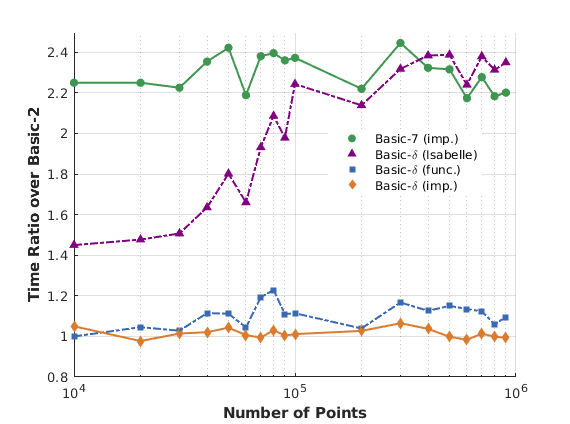
\includegraphics[width=0.8\textwidth]{./Benchmarks2.png}
\caption[]{Benchmarks.}
\label{fig:benchmark}
\end{figure}
%
\section{Conclusion} \label{section:conclusion}

We have presented the first verification (both functional correctness and running time) of two related
closest pair of points algorithms in the plane, without assuming the \isa{x} coordinates of all points
to be distinct. The executable code generated from the formalization is competitive with existing
reference implementations. A challenging and rewarding next step would be to formalize and verify a
closest pair of points algorithm in arbitrary dimensions. This case is treated rather sketchily in the literature.

\paragraph{Acknowledgements}
Research supported by DFG grants NI 491/16-1 and 18-1.%
\end{isamarkuptext}\isamarkuptrue%
%
\isadelimtheory
%
\endisadelimtheory
%
\isatagtheory
%
\endisatagtheory
{\isafoldtheory}%
%
\isadelimtheory
%
\endisadelimtheory
%
\end{isabellebody}%
\endinput
%:%file=~/Documents/Code/Isabelle/closestpair/Paper.thy%:%
%:%110=86%:%
%:%111=87%:%
%:%112=88%:%
%:%113=89%:%
%:%114=90%:%
%:%115=91%:%
%:%116=92%:%
%:%117=93%:%
%:%118=94%:%
%:%119=95%:%
%:%120=96%:%
%:%121=97%:%
%:%122=98%:%
%:%123=99%:%
%:%124=100%:%
%:%125=101%:%
%:%126=102%:%
%:%127=103%:%
%:%128=104%:%
%:%129=105%:%
%:%130=106%:%
%:%131=107%:%
%:%132=108%:%
%:%133=109%:%
%:%134=110%:%
%:%135=111%:%
%:%136=112%:%
%:%137=113%:%
%:%138=114%:%
%:%139=115%:%
%:%140=116%:%
%:%141=117%:%
%:%142=118%:%
%:%143=119%:%
%:%144=120%:%
%:%145=121%:%
%:%146=122%:%
%:%147=123%:%
%:%148=124%:%
%:%149=125%:%
%:%150=126%:%
%:%151=127%:%
%:%152=128%:%
%:%153=129%:%
%:%154=130%:%
%:%155=131%:%
%:%156=132%:%
%:%157=133%:%
%:%158=134%:%
%:%159=135%:%
%:%160=136%:%
%:%161=137%:%
%:%162=138%:%
%:%163=139%:%
%:%164=140%:%
%:%165=141%:%
%:%166=142%:%
%:%167=143%:%
%:%168=144%:%
%:%169=145%:%
%:%170=146%:%
%:%171=147%:%
%:%172=148%:%
%:%173=149%:%
%:%174=150%:%
%:%175=151%:%
%:%176=152%:%
%:%177=153%:%
%:%178=154%:%
%:%179=155%:%
%:%180=156%:%
%:%181=157%:%
%:%182=158%:%
%:%183=159%:%
%:%184=160%:%
%:%185=161%:%
%:%186=162%:%
%:%187=163%:%
%:%188=164%:%
%:%189=165%:%
%:%190=166%:%
%:%191=167%:%
%:%192=168%:%
%:%193=169%:%
%:%194=170%:%
%:%195=171%:%
%:%196=172%:%
%:%197=173%:%
%:%198=174%:%
%:%199=175%:%
%:%200=176%:%
%:%201=177%:%
%:%202=178%:%
%:%203=179%:%
%:%204=180%:%
%:%205=181%:%
%:%206=182%:%
%:%207=183%:%
%:%208=184%:%
%:%209=185%:%
%:%210=186%:%
%:%211=187%:%
%:%212=188%:%
%:%213=189%:%
%:%214=190%:%
%:%215=191%:%
%:%216=192%:%
%:%217=193%:%
%:%218=194%:%
%:%219=195%:%
%:%220=196%:%
%:%221=197%:%
%:%222=198%:%
%:%223=199%:%
%:%224=200%:%
%:%225=201%:%
%:%226=202%:%
%:%227=203%:%
%:%228=204%:%
%:%229=205%:%
%:%230=206%:%
%:%231=207%:%
%:%232=208%:%
%:%233=209%:%
%:%234=210%:%
%:%235=211%:%
%:%236=212%:%
%:%237=213%:%
%:%238=214%:%
%:%239=215%:%
%:%240=216%:%
%:%241=217%:%
%:%242=218%:%
%:%243=219%:%
%:%244=220%:%
%:%245=221%:%
%:%246=222%:%
%:%247=223%:%
%:%248=224%:%
%:%252=225%:%
%:%253=226%:%
%:%254=227%:%
%:%255=228%:%
%:%256=229%:%
%:%257=230%:%
%:%258=231%:%
%:%259=232%:%
%:%260=233%:%
%:%261=234%:%
%:%262=235%:%
%:%263=236%:%
%:%264=237%:%
%:%265=238%:%
%:%266=239%:%
%:%267=240%:%
%:%268=241%:%
%:%269=242%:%
%:%270=243%:%
%:%271=244%:%
%:%272=245%:%
%:%273=246%:%
%:%274=247%:%
%:%278=248%:%
%:%279=249%:%
%:%280=250%:%
%:%281=251%:%
%:%282=252%:%
%:%286=253%:%
%:%287=254%:%
%:%288=255%:%
%:%289=256%:%
%:%290=257%:%
%:%291=258%:%
%:%292=259%:%
%:%293=260%:%
%:%294=261%:%
%:%295=262%:%
%:%296=263%:%
%:%297=264%:%
%:%298=265%:%
%:%299=266%:%
%:%300=267%:%
%:%301=268%:%
%:%302=269%:%
%:%303=270%:%
%:%304=271%:%
%:%305=272%:%
%:%306=273%:%
%:%307=274%:%
%:%308=275%:%
%:%309=276%:%
%:%310=277%:%
%:%311=278%:%
%:%312=279%:%
%:%313=280%:%
%:%314=281%:%
%:%315=282%:%
%:%320=283%:%
%:%321=284%:%
%:%322=285%:%
%:%323=286%:%
%:%324=287%:%
%:%325=288%:%
%:%326=289%:%
%:%327=290%:%
%:%328=291%:%
%:%329=292%:%
%:%330=293%:%
%:%331=294%:%
%:%332=295%:%
%:%333=296%:%
%:%334=297%:%
%:%335=298%:%
%:%336=299%:%
%:%337=300%:%
%:%338=301%:%
%:%339=302%:%
%:%340=303%:%
%:%341=304%:%
%:%342=305%:%
%:%343=306%:%
%:%344=307%:%
%:%345=308%:%
%:%346=309%:%
%:%347=310%:%
%:%348=311%:%
%:%349=312%:%
%:%350=313%:%
%:%351=314%:%
%:%352=315%:%
%:%353=316%:%
%:%354=317%:%
%:%355=318%:%
%:%356=319%:%
%:%357=320%:%
%:%358=321%:%
%:%359=322%:%
%:%360=323%:%
%:%361=324%:%
%:%362=325%:%
%:%363=326%:%
%:%364=327%:%
%:%365=328%:%
%:%366=329%:%
%:%367=330%:%
%:%368=331%:%
%:%369=332%:%
%:%370=333%:%
%:%371=334%:%
%:%372=335%:%
%:%373=336%:%
%:%374=337%:%
%:%375=338%:%
%:%376=339%:%
%:%377=340%:%
%:%378=341%:%
%:%379=342%:%
%:%380=343%:%
%:%381=344%:%
%:%382=345%:%
%:%383=346%:%
%:%384=347%:%
%:%385=348%:%
%:%386=349%:%
%:%387=350%:%
%:%395=351%:%
%:%396=352%:%
%:%397=353%:%
%:%398=354%:%
%:%399=355%:%
%:%401=356%:%
%:%402=357%:%
%:%403=358%:%
%:%404=359%:%
%:%405=360%:%
%:%406=361%:%
%:%407=362%:%
%:%408=363%:%
%:%409=364%:%
%:%410=365%:%
%:%411=366%:%
%:%412=367%:%
%:%413=368%:%
%:%414=369%:%
%:%415=370%:%
%:%416=371%:%
%:%417=372%:%
%:%418=373%:%
%:%419=374%:%
%:%420=375%:%
%:%421=376%:%
%:%422=377%:%
%:%423=378%:%
%:%424=379%:%
%:%425=380%:%
%:%426=381%:%
%:%427=382%:%
%:%428=383%:%
%:%429=384%:%
%:%430=385%:%
%:%431=386%:%
%:%432=387%:%
%:%433=388%:%
%:%434=389%:%
%:%435=390%:%
%:%436=391%:%
%:%437=392%:%
%:%438=393%:%
%:%439=394%:%
%:%440=395%:%
%:%441=396%:%
%:%442=397%:%
%:%443=398%:%
%:%444=399%:%
%:%445=400%:%
%:%446=401%:%
%:%447=402%:%
%:%448=403%:%
%:%449=404%:%
%:%450=405%:%
%:%451=406%:%
%:%452=407%:%
%:%453=408%:%
%:%454=409%:%
%:%455=410%:%
%:%456=411%:%
%:%457=412%:%
%:%458=413%:%
%:%459=414%:%
%:%460=415%:%
%:%461=416%:%
%:%462=417%:%
%:%463=418%:%
%:%464=419%:%
%:%465=420%:%
%:%466=421%:%
%:%467=422%:%
%:%468=423%:%
%:%469=424%:%
%:%470=425%:%
%:%471=426%:%
%:%472=427%:%
%:%473=428%:%
%:%474=429%:%
%:%475=430%:%
%:%476=431%:%
%:%477=432%:%
%:%478=433%:%
%:%479=434%:%
%:%480=435%:%
%:%481=436%:%
%:%482=437%:%
%:%483=438%:%
%:%484=439%:%
%:%485=440%:%
%:%486=441%:%
%:%487=442%:%
%:%488=443%:%
%:%489=444%:%
%:%490=445%:%
%:%491=446%:%
%:%492=447%:%
%:%493=448%:%
%:%494=449%:%
%:%495=450%:%
%:%496=451%:%
%:%497=452%:%
%:%498=453%:%
%:%499=454%:%
%:%500=455%:%
%:%501=456%:%
%:%502=457%:%
%:%503=458%:%
%:%504=459%:%
%:%505=460%:%
%:%506=461%:%
%:%507=462%:%
%:%508=463%:%
%:%509=464%:%
%:%510=465%:%
%:%511=466%:%
%:%512=467%:%
%:%513=468%:%
%:%514=469%:%
%:%515=470%:%
%:%516=471%:%
%:%517=472%:%
%:%518=473%:%
%:%519=474%:%
%:%520=475%:%
%:%521=476%:%
%:%522=477%:%
%:%523=478%:%
%:%524=479%:%
%:%525=480%:%
%:%526=481%:%
%:%527=482%:%
%:%528=483%:%
%:%529=484%:%
%:%533=485%:%
%:%534=486%:%
%:%535=487%:%
%:%536=488%:%
%:%537=489%:%
%:%538=490%:%
%:%539=491%:%
%:%540=492%:%
%:%541=493%:%
%:%542=494%:%
%:%543=495%:%
%:%544=496%:%
%:%545=497%:%
%:%546=498%:%
%:%547=499%:%
%:%548=500%:%
%:%549=501%:%
%:%550=502%:%
%:%551=503%:%
%:%552=504%:%
%:%553=505%:%
%:%554=506%:%
%:%555=507%:%
%:%556=508%:%
%:%557=509%:%
%:%558=510%:%
%:%559=511%:%
%:%560=512%:%
%:%561=513%:%
%:%562=514%:%
%:%563=515%:%
%:%564=516%:%
%:%565=517%:%
%:%566=518%:%
%:%567=519%:%
%:%568=520%:%
%:%569=521%:%
%:%570=522%:%
%:%571=523%:%
%:%572=524%:%
%:%573=525%:%
%:%574=526%:%
%:%575=527%:%
%:%576=528%:%
%:%577=529%:%
%:%578=530%:%
%:%579=531%:%
%:%580=532%:%
%:%581=533%:%
%:%582=534%:%
%:%583=535%:%
%:%584=536%:%
%:%585=537%:%
%:%586=538%:%
%:%587=539%:%
%:%588=540%:%
%:%589=541%:%
%:%590=542%:%
%:%591=543%:%
%:%592=544%:%
%:%593=545%:%
%:%594=546%:%
%:%595=547%:%
%:%596=548%:%
%:%597=549%:%
%:%598=550%:%
%:%599=551%:%
%:%600=552%:%
%:%601=553%:%
%:%602=554%:%
%:%603=555%:%
%:%604=556%:%
%:%605=557%:%
%:%606=558%:%
%:%607=559%:%
%:%608=560%:%
%:%609=561%:%
%:%610=562%:%
%:%611=563%:%
%:%612=564%:%
%:%613=565%:%
%:%614=566%:%
%:%615=567%:%
%:%616=568%:%
%:%617=569%:%
%:%618=570%:%
%:%619=571%:%
%:%620=572%:%
%:%621=573%:%
%:%622=574%:%
%:%623=575%:%
%:%624=576%:%
%:%625=577%:%
%:%626=578%:%
%:%627=579%:%
%:%628=580%:%
%:%629=581%:%
%:%630=582%:%
%:%631=583%:%
%:%632=584%:%
%:%633=585%:%
%:%634=586%:%
%:%635=587%:%
%:%636=588%:%
%:%637=589%:%
%:%638=590%:%
%:%639=591%:%
%:%640=592%:%
%:%641=593%:%
%:%642=594%:%
%:%643=595%:%
%:%644=596%:%
%:%645=597%:%
%:%646=598%:%
%:%647=599%:%
%:%648=600%:%
%:%649=601%:%
%:%650=602%:%
%:%651=603%:%
%:%652=604%:%
%:%656=605%:%
%:%657=606%:%
%:%658=607%:%
%:%659=608%:%
%:%660=609%:%
%:%661=610%:%
%:%662=611%:%
%:%663=612%:%
%:%664=613%:%
%:%665=614%:%
%:%666=615%:%
%:%667=616%:%
%:%668=617%:%
%:%669=618%:%
%:%670=619%:%
%:%671=620%:%
%:%672=621%:%
%:%673=622%:%
%:%674=623%:%
%:%675=624%:%
%:%676=625%:%
%:%677=626%:%
%:%678=627%:%
%:%679=628%:%
%:%680=629%:%
%:%681=630%:%
%:%682=631%:%
%:%683=632%:%
%:%684=633%:%
%:%685=634%:%
%:%686=635%:%
%:%687=636%:%
%:%688=637%:%
%:%689=638%:%
%:%690=639%:%
%:%691=640%:%
%:%692=641%:%
%:%693=642%:%
%:%694=643%:%
%:%695=644%:%
%:%696=645%:%
%:%697=646%:%
%:%698=647%:%
%:%699=648%:%
%:%700=649%:%
%:%701=650%:%
%:%702=651%:%
%:%703=652%:%
%:%704=653%:%
%:%705=654%:%
%:%706=655%:%
%:%707=656%:%
%:%708=657%:%
%:%709=658%:%
%:%710=659%:%
%:%711=660%:%
%:%712=661%:%
%:%713=662%:%
%:%714=663%:%
%:%715=664%:%
%:%716=665%:%
%:%717=666%:%
%:%718=667%:%
%:%719=668%:%
%:%720=669%:%
%:%721=670%:%
%:%722=671%:%
%:%723=672%:%
%:%724=673%:%
%:%725=674%:%
%:%726=675%:%
%:%727=676%:%
%:%728=677%:%
%:%729=678%:%
%:%730=679%:%
%:%731=680%:%
%:%732=681%:%
%:%733=682%:%
%:%734=683%:%
%:%735=684%:%
%:%736=685%:%
%:%737=686%:%
%:%738=687%:%
%:%739=688%:%
%:%740=689%:%
%:%741=690%:%
%:%742=691%:%
%:%743=692%:%
%:%744=693%:%
%:%745=694%:%
%:%746=695%:%
%:%747=696%:%
%:%748=697%:%
%:%749=698%:%
%:%750=699%:%
%:%751=700%:%
%:%752=701%:%
%:%753=702%:%
%:%754=703%:%
%:%755=704%:%
%:%756=705%:%
%:%757=706%:%
%:%758=707%:%
%:%759=708%:%
%:%760=709%:%
%:%761=710%:%
%:%762=711%:%
%:%763=712%:%
%:%764=713%:%
%:%765=714%:%
%:%766=715%:%
%:%767=716%:%
%:%768=717%:%
%:%769=718%:%
%:%770=719%:%
%:%771=720%:%
%:%772=721%:%
%:%773=722%:%
%:%774=723%:%
%:%775=724%:%
%:%776=725%:%
%:%777=726%:%
%:%778=727%:%
%:%779=728%:%
%:%780=729%:%
%:%781=730%:%
%:%782=731%:%
%:%783=732%:%
%:%784=733%:%
%:%785=734%:%
%:%786=735%:%
%:%787=736%:%
%:%788=737%:%
%:%789=738%:%
%:%790=739%:%
%:%791=740%:%
%:%795=741%:%
%:%796=742%:%
%:%797=743%:%
%:%798=744%:%
%:%799=745%:%
%:%800=746%:%
%:%801=747%:%
%:%802=748%:%
%:%803=749%:%
%:%804=750%:%
%:%805=751%:%
%:%806=752%:%
%:%807=753%:%
%:%808=754%:%
%:%809=755%:%
%:%810=756%:%
%:%811=757%:%
%:%812=758%:%
%:%813=759%:%
%:%814=760%:%
%:%815=761%:%
%:%816=762%:%
%:%817=763%:%
%:%818=764%:%
%:%819=765%:%
%:%820=766%:%
%:%821=767%:%
%:%822=768%:%
%:%823=769%:%
%:%824=770%:%
%:%825=771%:%
%:%826=772%:%
%:%827=773%:%
%:%828=774%:%
%:%829=775%:%
%:%830=776%:%
%:%831=777%:%
%:%832=778%:%
%:%833=779%:%
%:%834=780%:%
%:%835=781%:%
%:%836=782%:%
%:%837=783%:%
%:%838=784%:%

\section{Related Work}

Cite related work.

\paragraph{Acknowledgement}
XYZ helped.

\bibliographystyle{splncs04}
\bibliography{root}

\end{document}
